\documentclass[12pt,a4paper,twoside]{report}
\usepackage[utf8]{inputenc}
\usepackage[english]{babel}
\usepackage{setspace}
\usepackage{amssymb,amsmath,amsfonts}
\usepackage{graphicx}
\usepackage{upquote} % quotes in verbatim environments
\usepackage{fixme}
\usepackage{microtype}
\usepackage[tmargin=3cm, lmargin=3cm, rmargin=3cm, bmargin=3cm, marginparsep=0.3cm, marginparwidth=2.4cm]{geometry}
\usepackage{hyperref}
\usepackage{import}
\PassOptionsToPackage{usenames,dvipsnames}{color} % color is loaded by hyperref
\hypersetup{unicode=true,
            colorlinks=true,
            linkcolor=black,
            citecolor=black,
            urlcolor=blue,
            breaklinks=true}
\urlstyle{same}  % don't use monospace font for urls
\usepackage{parskip}
\setlength{\emergencystretch}{3em}

\usepackage{algorithm}
\usepackage[end]{algpseudocode}
\let\Algorithm\algorithm
\renewcommand\algorithm[1][]{\Algorithm[#1]\setstretch{1.25}}

\usepackage[plain]{fancyref}
% Change references from capital/normal letters
\newcommand{\ffref}{\Fref}
% Algorithm and subsection references
\newcommand*{\fancyrefalglabelprefix}{alg}
\newcommand*{\fancyrefsubseclabelprefix}{subsec}
\frefformat{plain}{\fancyrefalglabelprefix}{%
algorithm\fancyrefdefaultspacing#1%
}
\Frefformat{plain}{\fancyrefalglabelprefix}{%
Algorithm\fancyrefdefaultspacing#1%
}
\frefformat{plain}{\fancyrefsubseclabelprefix}{%
subsection\fancyrefdefaultspacing#1%
}
\Frefformat{plain}{\fancyrefsubseclabelprefix}{%
Subsection\fancyrefdefaultspacing#1%
}
\frefformat{vario}{\fancyrefalglabelprefix}{%
algorithm\fancyrefdefaultspacing#1 on page~#2%
}
\Frefformat{vario}{\fancyrefalglabelprefix}{%
Algorithm\fancyrefdefaultspacing#1 on page~#2%
}
\frefformat{vario}{\fancyrefsubseclabelprefix}{%
subsection\fancyrefdefaultspacing#1 on page~#2%
}
\Frefformat{vario}{\fancyrefsubseclabelprefix}{%
Subsection\fancyrefdefaultspacing#1 on page~#2%
}

\usepackage{algpseudocode}
\algblockdefx[RepeatComment]{RepeatComment}{EndRepeatComment}
    [1][]{\textbf{repeat} #1}
    {\textbf{end repeat}}
\algblockdefx[RepeatUntilComment]{RepeatUntilComment}{EndRepeatUntilComment}
    [1][]{\textbf{repeat} #1}
    [1][]{\textbf{until} #1}

\usepackage{fancyhdr}
\setlength{\headheight}{15pt}
\fancyfoot{}
\fancyhead{}
\fancyhead[LE,RO]{\thepage}
\fancyhead[RE]{\nouppercase{\leftmark}}
\fancyhead[LO]{\nouppercase{\rightmark}}

%% Bibtex
\usepackage{csquotes}
%\usepackage[nottoc,numbib]{tocbibind}
\usepackage[numbib]{tocbibind}
\usepackage[style=authoryear,bibencoding=ascii,backend=bibtex,natbib]{biblatex}
\addbibresource{report.bib}

%% Inkscape pdf_tex pictures
\usepackage{calc}
\def\svgscale{1}
\newcommand{\inkscapefig}[2]{
\begin{figure}[hbtp]
\begin{center}
  \subimport{img/}{#1.pdf_tex}
\end{center}
\caption{#2\label{fig:#1}}
\end{figure}
}

\usepackage[final]{pdfpages}

\usepackage{mfirstuc} % capitalisewords

%\newcommand{\newconceptspec}[2]{\emph{#1}\marginpar{\footnotesize\textsc{#2}}}
\newcommand{\newconceptspec}[2]{\emph{#1}}
\newcommand{\newconcept}[1]{\newconceptspec{#1}{\capitalisewords{#1}}}
\newcommand{\centeredtitle}[1]{\begin{center} {\Huge \textbf{#1}}
    \addcontentsline{toc}{chapter}{#1} \end{center}\bigskip}
\newcommand{\argmin}{\operatornamewithlimits{arg\,min}}
\newcommand{\argmax}{\operatornamewithlimits{arg\,max}}

\subimport{Content/}{Acronyms.tex}

\begin{document}
\pagenumbering{roman}
\pagestyle{empty}
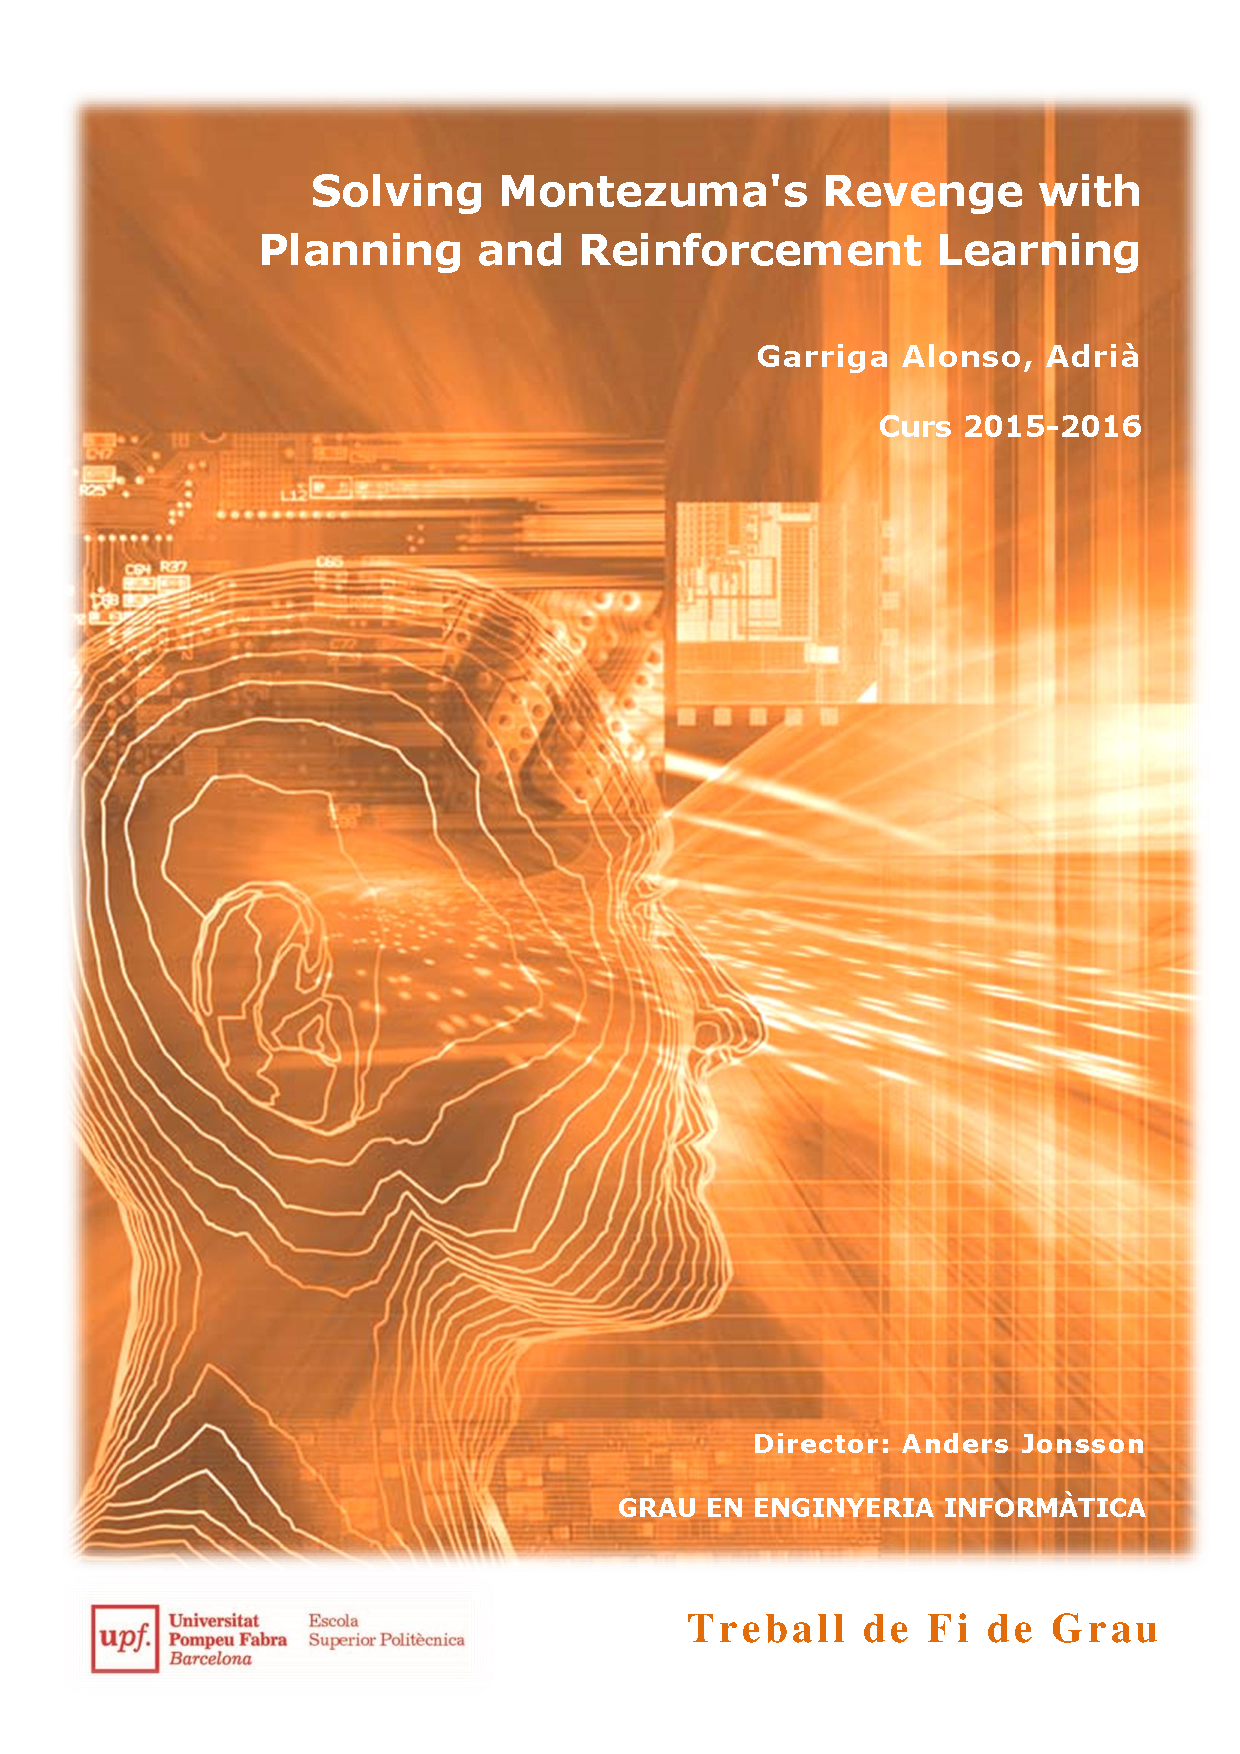
\includepdf[pages={1}]{Content/cover.pdf}
\cleardoublepage
\hypersetup{linkcolor=black}
\def\title{Solving Montezuma's Revenge with planning and reinforcement learning}
\def\subject{Planning \& Reinforcement Learning}
\def\keywords{Artificial Intelligence, Reinforcement Learning, Planning,
  Hierarchical Reinforcement Learning, Sparse, Intrinsic Motivation}
\def\date{\today}

\def\authorName{Adrià Garriga Alonso}
\def\authorEmail{adria.garriga01@estudiant.upf.edu}

\def\supervisorName{Anders Jonsson}
\def\supervisorEmail{anders.jonsson@upf.edu}

\def\departmentName{Department of Information and Communication Technologies}
\def\departmentWeb{http://www.upf.edu/dtic/en/}

\def\degree{Bachelor in Computer Science}
\def\univlogo{img/logo_upf.jpg}





\def\author{\texorpdfstring
  {\href{mailto:\authorEmail}{\authorName}}
  {\authorName}
}
\def\supervisor{\texorpdfstring
  {\href{mailto:\supervisorEmail}{\supervisorName}}
  {\supervisorName}
}
\def\department{\texorpdfstring
  {\href{\departmentWeb}{\departmentName}}
  {\departmentName}
}

\hypersetup{pdftitle={\title}}
\hypersetup{pdfsubject=\subject}
\hypersetup{pdfauthor=\author}
\hypersetup{pdfkeywords=\keywords}
\pagestyle{empty}
\begin{titlepage}
  \let\footnotesize\small
  \let\footnoterule\relax
  \let \footnote \thanks
  \setcounter{footnote}{0}
  \null\vfil
  \vskip 60pt
  \begin{center}
    \setlength{\parskip}{0pt}
    %{\large\textbf{\UNIVNAME}\par}
    %\vfill
    {\huge \bf \title \par}
    \bigskip
    \bigskip
    \bigskip
    %{\large by \par}
    \smallskip
    {\Large \author \par}
    \bigskip
    {\Large Supervised by \supervisor}
    \vfill
    {\Large \date \par}
    \vfill
    {\large \degree \par}
    \bigskip
    %{\large in the \par}
    %{\large \facname \par}
    {\large \department \par}
    \vfill
    \includegraphics[width=200px,height=100px, keepaspectratio]{\univlogo}
  \end{center}
%  \par
%  \@thanks
%  \vfil\null
\end{titlepage}
%\setcounter{footnote}{0}%
%\global\let\thanks\relax
%\global\let\maketitle\relax
%\global\let\thanks\@empty
%\global\let\author\@empty
%\global\let\date\@empty
%\global\let\title\@empty
%\global\let\title\relax
%\global\let\author\relax
%\global\let\date\relax
%\global\let\and\relax
\cleardoublepage

\onehalfspacing

\cleardoublepage
\newpage
\thispagestyle{empty}
\vfill
\centeredtitle{Acknowledgements}

To my supervisor Anders Jonsson, for the guidance offered in navigating the
literature, in carrying out this project. I also want to thank him for getting
me interested into the fascinating field of \acs{RL}.

To my good friend and upperclassman Daniel Furelos, for being an academic role
model to follow, and for the offered advice.

To my parents and sister for the moral support, and the support of a noisy,
electricity-hungry computer that is continuously learning and planning.

Thank you all!
\vfill

\cleardoublepage
\newpage
\thispagestyle{empty}
\vfill
\centeredtitle{Abstract}
Traditionally, methods for solving \acp{SDP} have not
worked well with those that feature sparse feedback. Both planning and
reinforcement learning, methods for solving \acp{SDP}, have trouble with sparse
feedback.

With the rise to prominence of the \ac{ALE} in the
broader research community of sequential decision processes, one \ac{SDP} featuring
sparse feedback has become familiar: the Atari game \acl{MR}. In this
particular game, the great amount of knowledge the human player already
possesses, and uses to find rewards, cannot be bridged by blindly exploring in a
realistic time.

We apply planning, hierarchical reinforcement learning and hybrid approaches,
combined with domain knowledge, to enable an agent to obtain better scores in
this game.

We hope that these domain-specific algorithms can inspire better approaches to
solve \acp{SDP} with sparse feedback in general.
\vfill

\cleardoublepage
%\lhead{Contents}
\pagestyle{fancy}
\tableofcontents
\pagestyle{empty}

%\cleardoublepage
%\lhead{List of Figures}
%\listoffigures

%\cleardoublepage
%%\lhead{List of Tables}
%\listoftables

\cleardoublepage
\pagestyle{empty}
\printacronyms[include-classes=abbrev,name=Abbreviations,heading=chapter*]
\addcontentsline{toc}{chapter}{Abbreviations}

\cleardoublepage
\pagestyle{fancy}
\pagenumbering{arabic}
\chapter{Introduction}
\section{The problem}
Us \emph{homo sapiens} are notoriously proud of our intelligence. Intelligence
is what allows us to handle the world we live in: understand our surroundings,
predict the future, and manipulate it according to our will. What will happen
if I move my hand to a pen and put my fingers around it? I will grasp it, and
then using my muscles I will be able to use it.

It is not at all obvious how we perform this process. Indeed, this question
has been philosophised on for thousands of years. The field of \ac{AI} tries
to go even further: researchers try understand how we think, in order to build
machines that exhibit those same properties.

Work on \ac{AI} famously started on the summer of 1956 at Dartmouth College.
John McCarthy and others proposed that a ``2 month, 10 man study of articifial
intelligence'' would make ``significant advance in one or more of [how to make
machines use language, form abstractions and concepts, solve kinds of problems
now reserved for humans, and improve themselves] if a carefully selected group
of scientists work on it together for a summer''. \citep[Section~1.3]{russell2009aima}

60 years later, we are still working on all of these problems. But this spark
ignited the tinder, and people started working on all kinds of subproblems:
computer vision, robotics, machine learning, automatic reasoning, natural
language processing\dots

The one we are concerned about in this document is sequential decision-making.
How might an agent take decisions, that have consequences, in a changing world?
Much research in this topic has been done on classical games, such as checkers,
chess and go, and on video games. These problems provide domains where actions
have to be taken sequentially and have consequences on the future.

One, important and recent, of such advances appeared in 2015 in Nature. The
paper ``Human-level control through deep reinforcement learning''
\citep{mnih2015human} proposed a neural algorithm that played many of the
video-games in the Atari console, knowing only the buttons it has, the score and
the image, just like a human player. Their key contribution is the \ac{DQN}
algorithm, which is the successful application of deep convolutional neural
networks (used in computer vision) as a function approximator for \ac{RL}.

Of the Atari games, \acl{MR} is one that their agent has trouble playing. The
problem with this game is the \emph{sparsity} of the rewards: it is almost
impossible to get any positive feedback just by randomly hitting buttons on the
console. To successfully get feedback, an agent has to understand the objects on
the screen, understand what is their character and how does it move, and then
purposefully plan a path to the rewards. Thus, the game has become infamous as
difficult, and many \ac{RL} researchers are interested in it now.

In this thesis we get around the problem of understanding the world by encoding
our own, human, understanding in the machine. It is an exercise to find out how
much must the machine know about the world, how few \emph{assumptions} must it
make, in order to be successful in it.

\section{Related Work}
Two very relevant papers have been recently published. They both deal with
methods intrinsic to the agent of obtaining more frequent feedback.

The first, by
\citet{kulkarni2016hierarchical}, proposes a hierarchical model
(\ffref{sec:hierarchical-rl}) with two levels. The higher level, the
\emph{meta-controller}, learns and decides towards which object of the screen
the character should move, and the lower level, the \emph{controller} learns and
decides how to get there. They encode the knowledge of which are plausible
objects to move towards and where is their controllable character to the
computational agent.

Some of the objects are closer to the initial position than the objects that
increase score in the game, so the controller can get some feedback and learn
how to move. Once the controller can move between objects, the objects which
produce reward are only a few abstract time steps away for the meta-controller,
and it can successfully learn too. Work on replicating this paper is in
progress.

The second, by \citet{bellemare2016unifying}, deals with estimating how
\emph{novel} (not to be confused with the novelty measure in
\ffref{subsec:iw-the-algorithm}) a state is, even if the agent has never seen
it. This is done by examining the components of the new state (like in
\ffref{subsec:iterated-width}) and the number of occurrences of each previous
component, and computing a single number synthesising that. Additional reward is
then given to visited states, proportional to the square root of this measure.
Thus, the learner is incentivised to visit new state areas, and eventually find
the environment reward in them.


%%% Local Variables: 
%%% mode: latex
%%% TeX-master: "../report"
%%% End: 

\cleardoublepage
\chapter{Background}
The immediate aim of this thesis is to produce a computer program that plays
\acl{MR} well. This problem statement suffices for most communication purposes,
but does not give us enough understanding to reason about the problem and find
ways to solve it. We first need to develop a formal definition of all the
notions: ``to play'', ``\acl{MR}'' and ``well''. We also need ways to know what
to do to play well. Fortunately, most of the required work has already been
done, by other authors.

In this chapter we will define mathematical models for the problem we are
facing. We will also formally define the algorithms we will use to tackle it,
without concerning ourselves with the details of their implementation on our
computing environment.

\section{\aclp{SDP}}
In this section, we describe the \acf{SDP} and related models. Most of the
definitions are taken from the \acl{RL} reference textbook,
\cite{sutton1998introduction}. Some are from the \ac{AI} textbook,
\cite{russell2009aima}. Concrete citations will be given after some claims, but
otherwise assume the concepts are taken from the first book.

Let us describe the \ac{SDP} model from
(\cite[Section~3.1]{sutton1998introduction}). There is an \newconcept{agent} that, every
\newconcept{time step}, takes an \newconcept{action} in the \newconcept{environment}. The
environment is a process that has a \newconcept{state}. When the agent takes an
action, the environment's state changes. The agent also receives a \newconcept{reward}
when it takes an action.

More formally. There is a series of discrete time steps, $t=0,1,2,3,\dots$, in
which the agent and the environment interact. At time step $t$, environment is
in state $s_t \in \mathcal{S}$. $\mathcal{S}$ is the finite, but usually very
large, set of possible states. The agent takes an action $a_t$ from the set of
possible actions in the state, $a_t \in \mathcal{A}_{s_t}$. In the next time
step, the agent receives a numerical reward $r_{t+1} \in \mathfrak{R}$, and the
environment transitions to a new state $s_{t+1} \in \mathcal{S}$.

The environment defines the set of possible states $\mathcal{S}$, the possible
actions in each state, which belong to the set of all possible actions
$\mathcal{A}_s \subseteq \mathcal{A}$, the reward for each state $\mathcal{S}$
and the rules for transitioning to the new state in each time step. The agent
simply chooses the action $a_t$ in each time step. The interaction between agent
and environment is illustrated in figure \ref{fig:agent-environment}.

\inkscapefig{agent-environment}{Diagram of interaction between agent and
  environment (\cite[Section~3.1]{sutton1998introduction})}

This model is really flexible. It does not constrain time steps to have the same
length, so each can represent a decision branching point and not actual time. An
example of this can be observed in go, chess, poker and others, where each move
takes a different amount of wall clock time. It is also not constrained how a new
state is chosen after an action: it may depend on anything, maybe even be
stochastic and not deterministic.

The model also accepts different abstraction levels of states and actions: in a
video game, they can be raw pixel data and controller input, or entity position
representation and moving to a certain screen. This idea is the basis of
hierarchical reinforcement learning, which is explained in section
\ref{section:hierarchical-rl}.

It is important to understand that the agent is only the \emph{process} that
\emph{decides} actions, not a physical object or entity. In the case of a robot, the
agent is only the controlling program: the actuators, mechanisms and sensors are part
of the environment. In the case of a video game, the code that emulates
the world and accepts controls is the environment, and the code that trains a
model or plans actions is the agent. This is the case even if the actions to be
taken are high-level, and not settings of force or torque on actuators or
muscles.

Observe also that the reward is usually computed by the agent process itself,
rather than given by the environment as the model description implies. However,
in our formal model it is external to the agent, because the agent cannot change
the reward function.

The model so far maps to two the notions we needed: ``\acl{MR}'' is the environment,
``to play'' is to run the process so that the agent chooses actions.
\subsection{Considerations and characteristics of \acp{SDP}}
We may also call an \ac{SDP} a \newconcept{task}, when we are emphasising its nature
as a problem that the agent has to solve.

In this whole work we assume all \aclp{SDP} are \newconcept{fully observable}. That
is, the agent's sensations fully determine which state the environment is in. In
general, that may not be the case. However, the formally defined notions cover
only this case.

\subsubsection{Finite and infinite \acp{SDP}}
An \ac{SDP} is \newconcept{finite} if the set of states $\mathcal{S}$ and the
set of possible actions, $\mathcal{A}$, are finite. Otherwise, it is
\newconcept{infinite}. We will treat only finite \acp{SDP} in this work.

\subsubsection{Episodic and continuing \acp{SDP}}
Sometimes it makes sense to divide a task in non-overlapping continued
interactions between the agent and environment. Such tasks are called
\newconcept{episodic}, and they have one final time step. In contrast,
\newconcept{continuing} tasks never stop, in theory.
(\cite[Section~3.3]{sutton1998introduction})

\subsubsection{Deterministic and stochastic \acp{SDP}}
We have not yet mentioned how the next state of an \ac{SDP} is determined. In
general, the next state is drawn from a probability distribution over all
possible states $\mathcal{S}$, that depends on the past history of actions,
states and rewards.

Sometimes, the probability distribution has all its weight on a single
state, that is, the next state is a function of the previous history of the
process. Such \acp{SDP} are called \newconcept{deterministic}. When a \ac{SDP} is not
deterministic, it is \newconcept{stochastic}.

\subsection{Returns}
What is to play ``well''? The agent's goal is, informally, to maximise the rewards it
gets. In general, we maximise the expected future reward at any time step,
that is, the expected \newconcept{return} at time $t$, $R_t$.
We could simply define $R_t$ as the sum of all rewards until the last time step, $T$:
\begin{equation}
  R_t = r_{t+1} + r_{t+2} + \dots + r_T
  \label{eq:undiscounted-reward}
\end{equation}

However, we may be faced with a continuing task, and the final time step may be
infinity. We could very well be faced with infinite return for each action.
If we want to pick the action with maximal return, and all actions have an
infinite return, we are forced to pick one at random.

Instead, we use a more general notion, that of \newconcept{discounted return}:
\begin{equation}
  R_t = r_{t+1} + \gamma r_{t+2} + \gamma^2 r_{t+3} + \dots = \sum_{k=0}^\infty
\gamma^k r_{t+k+1}
\end{equation}
Where $\gamma$, the \newconcept{discount rate}, is a parameter, $0 \leq \gamma \leq
1$. Observe that, if $\gamma=1$, the return is simply the sum of all rewards, as
in equation \ref{eq:undiscounted-reward}. If $\gamma<1$, however, we solve our
infinite return problem: as the time step approaches infinity, the weight its
reward is scaled by approaches zero, and $R_t$ converges.
(\cite[Subsection~17.1.1]{russell2009aima})

\subsection{\aclp{MDP}}
The \ac{SDP} formalism is not really used in practice. \acfp{MDP}, which are a
restricted case of \acp{SDP}, are used instead.

In general, the next state of an \ac{SDP} may depend on all the past states,
actions and rewards. A \acl{MDP} is a \acl{SDP} that follows the Markov property
(\cite[Section~3.5]{sutton1998introduction};
\cite[Section~17.1]{russell2009aima}), defined as follows.

\begin{equation}
  P \lbrace s_{t+1} = s, r_{t+1} = r | s_t,a_t,r_t,s_{t-1},a_{t-1}, \dots, r_1, s_0, a_0 \rbrace =
  P \lbrace s_{t+1} = s, r_{t+1} = r | s_t,a_t \rbrace
\end{equation}

That is, for all $s\in\mathcal{S}$ and $r\in\mathfrak{R}$, the probability that
in the next step the state is $s$ and the reward is $r$ is the same, whether
conditioned on the whole history of past states, actions and rewards, or
conditioned only on the current state and action. More concisely, the
probability distribution over the next possible states and rewards depends only
on the current state and action.

This property enables us to develop agents that choose an action
based only on the current state: in any \ac{MDP}, this decision is just as good as
considering all past states, actions and rewards.

Additionally, algorithms and additional theory developed on top of \acp{MDP} can
be easily adapted to any \ac{SDP}. Turning an \ac{SDP} into an \ac{MDP} is
trivial: let the state $s'_t$ of the \ac{MDP} be the sequence of current and
previous states, actions and rewards of the SDP, $s_t,a_t,r_t,s_{t-1},\dots,s_n$. If the
\ac{SDP} depends on all of its history $n=0$, otherwise we can take data until
$n=t-m$. Indeed, the latter, excluding rewards, is the approach taken in
\cite{mnih2015human}; \cite{kulkarni2016hierarchical}; and this thesis.

It is also possible for the state to encode an abstracted representation of the
past actions and sensations. A repairer agent includes in its state the size of
the screwdriver it grabbed a few seconds ago, not the sensations, actions and
rewards it had while performing such task.

We usually specify an \ac{MDP} task with the tuple $\langle \mathcal{S}, \mathcal{A}_s,
\mathcal{P}^a_{ss'}, \mathcal{R}^a_{ss'}, \gamma \rangle$:
(based on \cite[Section~3.6]{sutton1998introduction})
\begin{itemize}
\item The set of possible states, $\mathcal{S}$.
\item The available actions for each state, as a function of the state,
  $\mathcal{A}_s$. Some formulations use the set of possible actions
  $\mathcal{A}$ instead.
\item The matrix of transition probabilities from each state to another, given
  an action, $\mathcal{P}^a_{ss'} = P(s_{t+1}=s' | s_t=s, a_t=a)$.
\item The expected reward given a state, an action and the next state,
 $\mathcal{R}^a_{ss'} = E \lbrace r_{t+1} | s_t=s, a_t=a, s_{t+1}=s' \rbrace$
\item The discount factor for calculating returns, $\gamma$
\end{itemize}

Note that we lose the information of the probability distribution of rewards.

The $\mathcal{P}^a_{ss'}$ and $\mathcal{R}^a_{ss'}$ matrices are usually
intractably big, and indeed may be infinite if the \ac{MDP} is infinite.

\section{Optimal decision-making in SDP}
\subsection{Policies and value functions}
A \newconcept{policy} $\pi$ is a probability distribution for each state
$s\in\mathcal{S}$, over the possible actions to take $a \in \mathcal{A}_s$. It
is represented as a probability associated to each state-action pair: $P =
\pi(s, a)$. We may also write $a = \pi(s)$, if the policy is deterministic:
$\pi(s, a')=1$ if $a'=a$ and $\pi(s, a')=0 if  a' \neq a$.

A \newconcept{value} $V^\pi(s)$ is the expected return for an agent following the
policy $\pi$, that is currently in state $s$. We define it as follows:
\begin{equation}
  V^\pi(s) = E_\pi \lbrace R_t | s_t = s \rbrace =
  E_\pi \left\{ \left. \sum_{k=0}^\infty \gamma^kr_{t+k+1} \right| s_t = s \right\}
  \label{eq:definition-value}
\end{equation}

We can also define the \newconcept{action-value function} $Q^\pi(s, a)$ of a policy
$\pi$, which is the expected return from taking action $a$ in state $s$ and
following $\pi$ thereafter.
\begin{equation}
  Q^\pi(s, a) = E_\pi \lbrace R_t | s_t = s, a_t = a \rbrace =
  E_\pi \left\{ \left. \sum_{k=0}^\infty \gamma^kr_{t+k+1} \right| s_t = s, a_t = a \right\}
  \label{eq:definition-qvalue}
\end{equation}

(\cite[Section~3.7]{sutton1998introduction})

We can calculate the value of a state by doing the average of the
expected values of all the actions, weighted by the probability of each action
being taken.The probability of each action being taken is determined by the
policy, so we get the following identity:
\begin{equation}
  \begin{split}
  \sum_{a\in\mathcal{A}_s}\pi(s, a) Q^\pi(s, a) & = \sum_{a\in\mathcal{A}_s}\pi(s, a) E_\pi \lbrace R_t | s_t = s, a_t = a \rbrace \\
  & = E_\pi \lbrace R_t | s_t = s \rbrace = V^\pi(s)
  \end{split}
  \label{eq:equivalence-qvalue-value}
\end{equation}


\subsection{Optimal policy\label{subsection:optimal-policy}}

Some of the policies will have higher values than others. The policy with the
maximum value for a state is called the \newconcept{optimal policy} for that state,
denoted by $\pi^*_s$. The optimal policy for a state is that which maximises its utility.
\begin{equation}
\pi^*_s = \argmax_\pi V^\pi(s)
\end{equation}
It is also important that the optimal policy is independent of the state it
starts with, if we don't cut the return at a time-step before the final
time-step (that is, the \newconcept{horizon} is infinite) and we use discounted
returns. So, we can just write $\pi^*$ to refer to the optimal policy.

The value of a state when following the optimal policy, $V^{\pi^*}(s)$, is the
\newconcept{true value}, or optimal value, of a state. Thus, we will just write $V(s)$ to refer to it.

If we know the true value function of all the states and the transition model of
the environment, we can calculate the optimal policy:
\begin{equation}
  \pi^*(s) = \argmax_{a\in\mathcal{A}_s} \sum_{s'\in\mathcal{S}}\mathcal{P}^a_{ss'}V(s)
  \label{eq:optimal-policy-value}
\end{equation}

Notice that we wrote it as an action, function of only the state, and not as a
probability, function of both the state and the action. This is because optimal
policies take only one action. Or several, with equal probability, if they all
have the same, maximal, utility.

(\cite[Subsection~17.1.2]{russell2009aima})

\subsection{Bellman equations}
Both value and action-value functions satisfy a recursive relationship that is
very widely used in reinforcement learning algorithms: the Bellman equations.

Starting with equation \ref{eq:definition-value}, we separate the first reward
from the sum of future rewards to obtain the Bellman equation for values:
\begin{equation}
\begin{split}
  V^\pi(s) & = E_\pi \lbrace R_t | s_t = s \rbrace \\
  & = E_\pi \left\{ \left. \sum_{k=0}^\infty \gamma^kr_{t+k+1} \right| s_t = s \right\} \\
  & = E_\pi \left\{ \left. r_{t+1} + \gamma\sum_{k=0}^\infty \gamma^kr_{t+k+2} \right| s_t = s \right\} \\
  & = \sum_{a\in\mathcal{A}_s} \left( \pi(s, a) \sum_{s' \in \mathcal{S}}\mathcal{P}^a_{ss'}
\left[\mathcal{R}^a_{ss'} + \gamma E_\pi \left\{ \left. \sum_{k=0}^\infty
\gamma^kr_{t+k+2} \right| s_{t+1} = s' \right\} \right] \right) \\
  & = \sum_{a\in\mathcal{A}_s} \left( \pi(s, a) \sum_{s' \in \mathcal{S}}\mathcal{P}^a_{ss'}
\left[\mathcal{R}^a_{ss'} + \gamma V^\pi(s') \right] \right)
\end{split}
\label{eq:bellman-v}
\end{equation}

And let us do the same for action-values, starting with equation
\ref{eq:definition-qvalue}:

\begin{equation}
  \begin{split}
    Q^\pi(s, a) & = E_\pi \lbrace R_t | s_t = s, a_t = a \rbrace \\
    & = E_\pi \left\{ \left. \sum_{k=0}^\infty \gamma^kr_{t+k+1} \right| s_t = s, a_t = a \right\} \\
    & = E_\pi \left\{ \left. r_{t+1} + \gamma\sum_{k=0}^\infty \gamma^kr_{t+k+2} \right| s_t = s, a_t = a \right\} \\
    & = \sum_{s' \in \mathcal{S}}\mathcal{P}^a_{ss'} \left[\mathcal{R}^a_{ss'} +
      \gamma E_\pi \left\{ \left. \sum_{k=0}^\infty \gamma^kr_{t+k+2} \right| s_{t+1}
        = s' \right\} \right] \\
    & = \sum_{s' \in \mathcal{S}}\mathcal{P}^a_{ss'}
    \left[\mathcal{R}^a_{ss'} + \gamma V^\pi(s') \right]
  \end{split}
\end{equation}

(\cite[Section~3.7]{sutton1998introduction})

And if we then substitute in equation \ref{eq:equivalence-qvalue-value}:
\begin{equation}
  Q^\pi(s, a) = \sum_{s' \in \mathcal{S}}\mathcal{P}^a_{ss'}
    \left[\mathcal{R}^a_{ss'} + \gamma \sum_{a'\in\mathcal{A}_{s'}}\pi(s', a')Q^\pi(s', a') \right]
    \label{eq:bellman-q}
\end{equation}


\subsubsection{Bellman equations with the optimal policy}
Recall from equation \ref{eq:optimal-policy-value} that the optimal policy takes
the action that maximises the true value of the next state. So, let's put this
notion into equation \ref{eq:bellman-v}:
\begin{equation}
  \begin{split}
  V(s) &= \sum_{a\in\mathcal{A}_s} \left( \pi^*(s, a)
    \sum_{s' \in \mathcal{S}}\mathcal{P}^a_{ss'}
    \left[\mathcal{R}^a_{ss'} + \gamma V^\pi(s') \right] \right) \\
  &= \max_{a\in\mathcal{A}_s}\sum_{s' \in \mathcal{S}}\mathcal{P}^a_{ss'}
\left[\mathcal{R}^a_{ss'} + \gamma V^\pi(s') \right]
  \end{split}
\label{eq:bellman-v-optimal}
\end{equation}
And equation \ref{eq:bellman-q}:
\begin{equation}
  \begin{split}
  Q(s, a) &= \sum_{s' \in \mathcal{S}}\mathcal{P}^a_{ss'}
    \left[\mathcal{R}^a_{ss'} + \gamma \sum_{a'\in\mathcal{A}_{s'}}\pi^*(s', a')Q^\pi(s', a') \right] \\
  &= \sum_{s' \in \mathcal{S}}\mathcal{P}^a_{ss'}
    \left[\mathcal{R}^a_{ss'} + \gamma \max_{a'\in\mathcal{A}_{s'}}Q^\pi(s', a') \right]
  \end{split}
\label{eq:bellman-q-optimal}
  \end{equation}
(\cite[Section~17.2.1]{russell2009aima}, \cite[Section~3.8]{sutton1998introduction})

These optimal Bellman equations are the basis of most modern reinforcement
learning algorithms.


\section{\acl{RL}}
Unless stated otherwise, concepts in this section are taken from
\cite{sutton1998introduction}. More concrete citations may also be given.

\acf{RL} is about an agent learning from experience how to behave to maximise
rewards over time. This experience is usually gathered by interacting with the
environment.

\subsection{\acl{VI}}
\acf{VI} is an algorithm, part of the Dynamic Programming collection of
algorithms for \ac{RL}. Those algorithms can compute optimal policies for an
\ac{MDP}, given a perfect model of the environment ($\mathcal{P}^a_{ss'}$,
$\mathcal{R}^a_{ss'}$, and the parameter $\gamma$).

\ac{VI} works by keeping a table with the values of all states, and
turning the optimal value Bellman equation (\ref{eq:bellman-v-optimal}) into an
update rule for the table. \ac{VI} is described in algorithm
\ref{alg:value-iteration}.

\begin{algorithm}
\begin{algorithmic}
\State Initialize $V(s)$ arbitrarily, for example $V(s)=0 \; \forall s\in\mathcal{S}$
\Repeat
  \State $\Delta \gets 0$, is the maximum update magnitude this iteration
  \For{each $s\in\mathcal{S}$}
    \State $v \gets V(s)$
    \State $V(s) \gets \max_{a\in\mathcal{A}_s}\sum_{s' \in \mathcal{S}}\mathcal{P}^a_{ss'} \left[\mathcal{R}^a_{ss'} + \gamma V^\pi(s') \right]$
    \State $\Delta \gets \max(\Delta, \left|V(s) - v \right| $
    \EndFor
\Until{$\Delta < \theta$ a small constant}
\State Output optimal policy using equation \ref{eq:optimal-policy-value}
\end{algorithmic}
\caption{\acl{VI} (\cite[Section~4.4]{sutton1998introduction})}
\label{alg:value-iteration}
\end{algorithm}

The value table kept in \ac{VI} is guaranteed to converge the true value $V^*$
under the same conditions that guarantee the existence of the latter

(\cite[Section~4.4]{sutton1998introduction})

There is another variant of \acl{VI}. In each outer iteration, we update only
one of the values in the table. As long as none of the values stops being
updated at a certain point in the computation, $V(s)$ will still converge to $V^*(s)$.

This does not decrease the amount of computation required to approximate the
optimal value function. However, sweeping over all states is often infeasible,
so this allows the algorithm to start making progress without having to do a
single whole sweep.

We can take advantage of this, and update more often the more promising states,
to be able to terminate \acl{VI} earlier and still have a good enough policy.
(\cite[Section~4.5]{sutton1998introduction})

 We could also just update the value of whatever state the agent ended up in
from the previous iteration, provided that we make the agent eventually visit
all states, and still converge to the optimal policy. This one of the basic
ideas in the Sarsa algorithm in subsection \ref{subsection:sarsa}, Q-learning,
\aclp{DQN} and many others similar in spirit.

\subsection{Exploration-exploitation and \texorpdfstring{$\varepsilon$}{ε}-greedy policies}
Agents that are interacting with an environment and learning while collecting
rewards face the \newconcept{exploration-exploitation tradeoff}. Should they take the
current maximum return action, or take an action with less return, that may turn
out to have a higher return when the internal value function is closer to the
optimal function?

One way to deal with this tradeoff is to follow an
\newconceptspec{$\varepsilon$-greedy policy}{$\varepsilon$-greedy Policy}.
Recall from subsection \ref{subsection:optimal-policy} that optimal policies,
and ``optimal'' policies based on a sub-optimal value function, always take one
action for any state. Instead of taking only that action, $\varepsilon$-greedy
policies:
\begin{itemize}
\item Take $\pi^*(s)$ with probability $1-\varepsilon$
\item Take an uniformly randomly sampled $a\in\mathcal{A}_s$ with probability
$\varepsilon$
\end{itemize}
Where $\varepsilon$ is a parameter, $0\leq\varepsilon\leq 1$. Often,
$\varepsilon=0.1$.

(\cite[Section~2.2]{sutton1998introduction})

\subsection{Sarsa\label{subsection:sarsa}}

Suppose an agent knows the optimal value function, $V(s)$, and is in state $s$.
How would it go about choosing its next action? Maybe it uses a
$\varepsilon$-greedy optimal policy as seen in the previous section, but
calculating the $\varepsilon$-greedy optimal policy requires calculating the
optimal policy.

\begin{equation}
  \pi^*(s) = \argmax_{a\in\mathcal{A}_s} \sum_{s'\in\mathcal{S}}\mathcal{P}^a_{ss'}V(s)
  \tag{\ref{eq:optimal-policy-value} revisited}
\end{equation}

Note that we need a model of the environment, $\mathcal{P}^a_{ss'}$, as well as the
value function $V(s)$. However, if we know the action-value function, we do not
need a model of the environment.
\begin{equation}
  \pi^*(s) = \argmax_{a\in\mathcal{A}_s} Q(s, a)
  \label{eq:q-policy}
\end{equation}

For this reason, methods that learn action-value functions are called
\newconcept{model-free methods} (\cite[Subsection~21.3.2]{russell2009aima}).

\begin{algorithm}[h]
\caption{Sarsa (\cite[Section~6.4]{sutton1998introduction})}
\label{alg:sarsa}
\begin{algorithmic}
\State Initialize $Q(s, a)$ arbitrarily, for example $Q(s, a)=0 \; \forall
s\in\mathcal{S}$
\RepeatComment{for each episode}
  \State Set $s$ to the current, initial, state
  \State Choose action $a$ for $s$, sampling from $a \sim \pi^\varepsilon_Q(s)$
  \RepeatUntilComment{for each step of episode}
    \State Take action $a$, observe reward $r$, state $s'$
    \State Choose action $a'$ for $s'$, sampling from $a' \sim \pi^\varepsilon_Q(s')$
    \State $Q(s, a) \gets (1-\alpha)Q(s,a) +
      \alpha \left[r + \gamma Q(s', a') \right]$ (update step)
    \State $s \gets s'$; $a \gets a'$
  \EndRepeatUntilComment{$s$ is terminal}
\EndRepeatComment
\end{algorithmic}
\end{algorithm}

$\pi^\varepsilon_Q$ is an $\varepsilon$-greedy policy based on
the optimal policy based on $Q$, as per equation \ref{eq:q-policy}. It is
possible to use other policies based on the optimal policy based on $Q$. However,
the policy used must have a non-zero probability of choosing all the actions for
convergence to the optimal policy to be guaranteed.

$\alpha$ is the \newconcept{learning rate}, $0\leq\alpha\leq 1$. Because we
don't have the model or policy, only \emph{samples} from them, we cannot
completely update our $Q$ following the Bellman equation. Thus, we instead
\emph{move our value towards} the $Q$-value based on the next one according to
something analogous to the Bellman equation, but we keep $(1-\alpha)$ of the old
value and only account for the new value weighted by $\alpha$.

Sarsa's name comes from the quintuple of values used in its update:
$\langle s_t, a_t, r_{t+1}, s_{t+1}, a_{t+1}\rangle$.

(\cite[Section~6.4]{sutton1998introduction})

\subsubsection{Function approximation}
For interesting problems, it is usually infeasible to store the $Q$ function for
all states and values. Instead, we use a learned function that approximates $Q$.
Desirable approximate functions not only store values close to those of the states and
actions the agent has seen, but also \emph{generalise} to unseen states and
actions. A very desirable method for learning such approximate functions is the
use of \acfp{NN}, and \acfp{DQN} (subsection \ref{subsection:dqn}) are a version
of Sarsa that use \acp{NN} for approximating the action-value function. 

When using function approximation in Sarsa, the only step changed is the $Q$
update step. Instead of updating a table with the learning rate, it updates the
function being learned, in a manner that depends on the function.

\subsection{Shaping}
Shaping is the practice of giving an agent intermediate rewards that are not
present in the environment. They aim to make learning easier by giving the agent
more frequent feedback. However, rewards added by shaping may change the
behaviour of the agent from what would be the optimal behaviour with the original
\ac{MDP}. Indeed, this happened while
conducting naive learning experiments with shaping for this work (subsection
\ref{subsection:reward-shaping}).

The following definitions and observations are taken from, and proved in,
\cite{ng1999policy}.

Let $\mathcal{M} = \langle \mathcal{S}, \mathcal{A},
\mathcal{P}^a_{ss'}, \mathcal{R}^a_{ss'}, \gamma \rangle$ be the \ac{MDP} the
agent interacts in. We change that \ac{MDP} for another one, $\mathcal{M}' = \langle
\mathcal{S}, \mathcal{A}, \mathcal{P}^a_{ss'}, \mathcal{R}'^a_{ss'}, \gamma
\rangle$, where $\mathcal{R}'^a_{ss'} = \mathcal{R}^a_{ss'} + F(s, a, s')$.
$F : \mathcal{S} \times A \times \mathcal{S} \mapsto \mathbb{R}$ is a bounded
real-valued function called the \newconcept{shaping function}.

Let $\phi(s)$, $\phi : \mathcal{S} \mapsto \mathbb{R}$ be a potential function.
A shaping function $F(s, a, s')$ does not alter the optimal policy if and only
if it is a \newconcept{potential-based function}. That is, there exists a
potential function $\phi$ such that:
\begin{equation}
  F(s, a, s') = \gamma \phi(s') - \phi(s)
\end{equation}

Potential-based reward functions are robust: near-optimal policies
in $\mathcal{M}$ remain near-optimal policies in $\mathcal{M'}$: if $\left|
V^\pi_M - V^*_M \right| < \varepsilon$, then $\left| V^\pi_{M'} - V^*_{M'}
\right| < \varepsilon$.

\section{Hierarchical Reinforcement Learning\label{section:hierarchical-rl}}

Suppose Alice wants to eat a salad. She needs the ingredients, so, she needs to
go to the grocery store. To accomplish that, she needs to get out of the house,
go out the door, \dots To accomplish the first, she needs to get up from the
chair, get out the room, and navigate to the front door. To get up from the
chair, she needs to tense her leg muscles in this way, move her arms in that
way, \dots

Like most if not all humans (and animals), Alice accomplishes tasks by taking
large abstract actions, that are divided into actions, that in turn are divided
into actions, and so on until she reaches contractions of muscle fibres.

Each sub-task can be learned and perfected individually, in all instances it is
performed. For example, learning to walk is useful for going to the grocery
store or going to school, and it gets perfected every time Alice (among other
things) goes to either of the two places.

\subsection{Options}

How may we encode this helpful intuition into reinforcement learning agents?
\cite{sutton1999between}, have an answer. The agent may take
\newconcept{options} instead of actions at every state. Options are courses of
action that last one or more time steps, and follow their own policy. Options take
other options and have their own policy, which can be improved every time they
are taken.

An option is a triple $\langle \mathcal{I}, \pi, \beta \rangle$:
\begin{itemize}
  \item $\mathcal{I} \subseteq \mathcal{S}$, the set of states the action can be
    \newconcept{initiated} the set of states the action can be
    \newconcept{initiated} in.
  \item $\pi(s, a)$, $\pi : \mathcal{S} \times \mathcal{A} \mapsto \mathbb{R}$,
the option's policy.
  \item $\beta(s)$, $\beta : \mathcal{S} \mapsto [0, 1]$, the probability that
the option is interrupted in state $s$.
\end{itemize}

The policy for an option only needs to be defined for a subset $S_o \subseteq
\mathcal{S}$ of the states, as we can define $\beta(s) = 1$ for $s \in S_o$.
Usually also, the action can be initiated wherever its policy is defined, that
is, $\mathcal{I} = S_o$

Normal actions are a special case of options, of duration 1 time step. The
option corresponding to an action $a$ is defined as follows:
\begin{itemize}
  \item $\mathcal{I} = \left\{ s \in \mathcal{S} | a \in \mathcal{A}_s \right\}$
  all the states the action can be taken in.
  \item $\pi(s, a') = 1$ if $a'=a$, otherwise $\pi(s, a') = 0$; for all
$s\in\mathcal{I}$.
  \item $\beta(s) = 1$ for all $s\in\mathcal{S}$.
\end{itemize}

\subsection{Semi-Markov options}
Sometimes it is desirable that actions end after a certain ``timeout'', as well
as in certain states, to avoid agents getting stuck. This case is accommodated
with \newconcept{semi-Markov options}, that depend on the whole history of
states, actions and rewards since they start.

Let a semi-Markov option start in time $t$ and ends in time $\tau$. We call the
sequence $s_t,a_t,r_t,s_{t+1},a_{t+1},\dots,r_\tau,s_\tau$ the
\newconcept{history}, denoted by $h_{t\tau}$. The set of all possible
$h_{t\tau}$ is $\Omega$

An semi-Markov option is a triple $\langle \mathcal{I}, \pi, \beta \rangle$,
with only $\pi$ and $\beta$ differing from the Markov option case:
\begin{itemize}
  \item $\pi(h, a)$, $\pi : \Omega \times \mathcal{A} \mapsto \mathbb{R}$,
the option's policy.
  \item $\beta(h)$, $\beta : \Omega \mapsto [0, 1]$, the probability that
the option is interrupted in state $s$.
\end{itemize}

Options that take other options as actions are semi-Markov, even if all the
underlying options are Markov options.

\subsection{\acfp{SMDP}}

A \ac{SMDP} is defined by:
\begin{itemize}
  \item A set of states $\mathcal{S}$.
  \item A set of actions. We call it $\mathcal{O}$, because this set will be the
    set of possible options in our case. Being a set of options, each has some
    possible initial states. We denote the options available in state $s$ as
$\mathcal{O}_s$.
  \item An expected cumulative discounted reward after taking action $o \in
    \mathcal{O}$ when in state $s \in \mathcal{S}$. We denote it by $r^o_s$. Let
    $t+k$ be the random time at which $o$ terminates. Let $\varepsilon(o, s, t)$
    be the event of option $o$ being initiated in state $s$ at time $t$. Then:
    \begin{equation}
      r^o_s = E\left\{ r_{t+1} + \gamma r_{t+2} + \gamma^2 r_{t+3} + \dots
      + \gamma^{k-1} r_{t+k} \right\}
    \end{equation}
  \item A well defined joint distribution of next state and transit time, $p(s,
    o, s', k)$, $p : \mathcal{S} \times \mathcal{O} \times \mathcal{S} \times
    \mathbb{N} \mapsto [0, 1]$. For our purposes, we only need $p^o_{ss'}$:
    \begin{equation}
      p^o_{ss'} = \sum_{k=1}^\infty p(s, o, s', k) \gamma^k
    \end{equation}
    This describes the likelihood of reaching a state $s'$ from state $s$ when
    taking option $o$, discounted depending on the time taken to reach it. The
    usefulness of this term will be apparent in the \ac{SMDP}'s Bellman equation
  (\ref{eq:smdp-bellman-q}).
  \item The discount factor $\gamma$.
\end{itemize}

So we treat it as the tuple $\langle \mathcal{S}, \mathcal{O}, r^o_s, p^o_{ss'},
\gamma\rangle$.

\subsection{Action-value Bellman equation and Sarsa}
The Bellman equation for action-values in \acp{SMDP} ends up looking very
similar to the one for \acp{MDP}.
\begin{equation}
  Q^\pi(s, o) = r^o_s + \sum_{s'}p^o_{ss'} \sum_{o' \in \mathcal{O}_{s'}} \pi(s', o')Q^\pi(s', o')
  \label{eq:smdp-bellman-q}
\end{equation}

The factor $p^o_{ss'}$ is useful because it incorporates both the probability of
reaching a state and the discount its action-value would incur. Thus, it is
exactly what the Q-value of the state we arrive in should be weighted by.

And of course, we take the maximum action-value if we are defining the optimal policy:
\begin{equation}
  Q^\pi(s, o) = r^o_s + \sum_{s'}p^o_{ss'} \max_{o' \in \mathcal{O}_{s'}} Q^*(s', o')
\end{equation}

The Sarsa update looks like this (analogous to the Q-learning update from
\cite[Section~3.2]{sutton1999between}):
\begin{equation}
  Q(s_t, o_t) \gets (1-\alpha)Q(s_t, o_t) + \alpha \left[r_{t:t+k} + \gamma^k Q(s_{t+k}, o_{t+k}) \right]
\end{equation}
Where $s_t$, $o_t$ are the currently selected state and option, $s_{t+k}$ and
$o_{t+k}$ are the next selected state and option, and $k$ is the number of time
steps between $s_t$ and $s_{t+k}$. $r_{t:t+k}$ is the cumulative discounted
reward over the indicated time range.

Note that all these expressions reduce to their ordinary \ac{MDP} counterparts
when the option corresponds to a primitive action.

%DIMARTS
\section{Planning}

Get ideas from \cite{russell2009aima}.
\subsection{Blind Planning}
BFS and friends
\subsection{Heuristic Planning}
A* and friends
\subsection{\acl{IW}}
nir ijcai
\subsection{Combining planning and learning}
we use our friendly neighbor \cite{sutton1998introduction}


%DIMECRES
\section{\aclp{NN}}
\subsection{Backpropagation}
\subsection{\aclp{CNN}}
\subsection{\aclp{DQN}\label{subsection:dqn}}

%%% Local Variables: 
%%% mode: latex
%%% TeX-master: "../report"
%%% End: 
\cleardoublepage
%DIJOUS
\newcommand{\refscreen}[1]{\hyperref[fig:montezuma-map]{screen~#1}}
\chapter{Methodology}
\section{\acl{MR}}
\subsection{Description}
You, the player, are Panama Joe, an intrepid explorer-archaeologist. Your latest
trip has brought you to discover the entrance to an Aztec pyramid. Filled with
excitement, you rush to search the treasures that surely await inside. But the
pyramid is full of traps and monsters. You will need all of your wits and agility to
get out alive!\footnote{Game background from the review by \citet{adair2007montezuma}.}

In the game, Panama Joe can run, jump and climb ladders, ropes and poles. The
pyramid he can explore is divided in 24 screens, numbered 0--23, depicted in
\ffref{fig:montezuma-map}. The player starts the game in screen 1 and ends when
collecting the gems in screen 15. When the player completes the game, it simply
resets with a different colour scheme.

Joe has a number of lives, initially 5. When they are over and Joe loses a life
again, the game is over. Lives can be lost by touching monsters, touching blue
wall traps (such as those in \refscreen{12}), falling
into quicksand pits or falling from too high.

The player can gain score for a number of things: collecting gems (+1000),
keys (+100), the sword (+100), the torch (+3000) or the mallet (+200); opening a
door (+300); or killing a monster with the sword (+2000). A life
is gained for every $10\,000$ points gained, with a maximum of 6 lives. The
torch allows you to see in the lowest floor of the pyramid (which is otherwise
black). The sword allows you to kill one monster. The mallet allows you to be
immune to monsters for a period of time.

The game can be rendered impossible to complete, since there are 6 doors but
only 4 keys. The two doors in \refscreen{17} need to be opened to finish, and
either one of the doors in \refscreen{1} needs to be opened to do almost
anything. So the player can either open both doors in \refscreen{1} and not see
in the bottom floor, or leave one door in each of the screens 1 and 4 unopened.

\begin{figure}[p]
\setlength{\unitlength}{\textwidth}
\begin{center}
%\noindent\makebox[\textwidth]{
  \begin{picture}(1,.513)
    \put(0,0){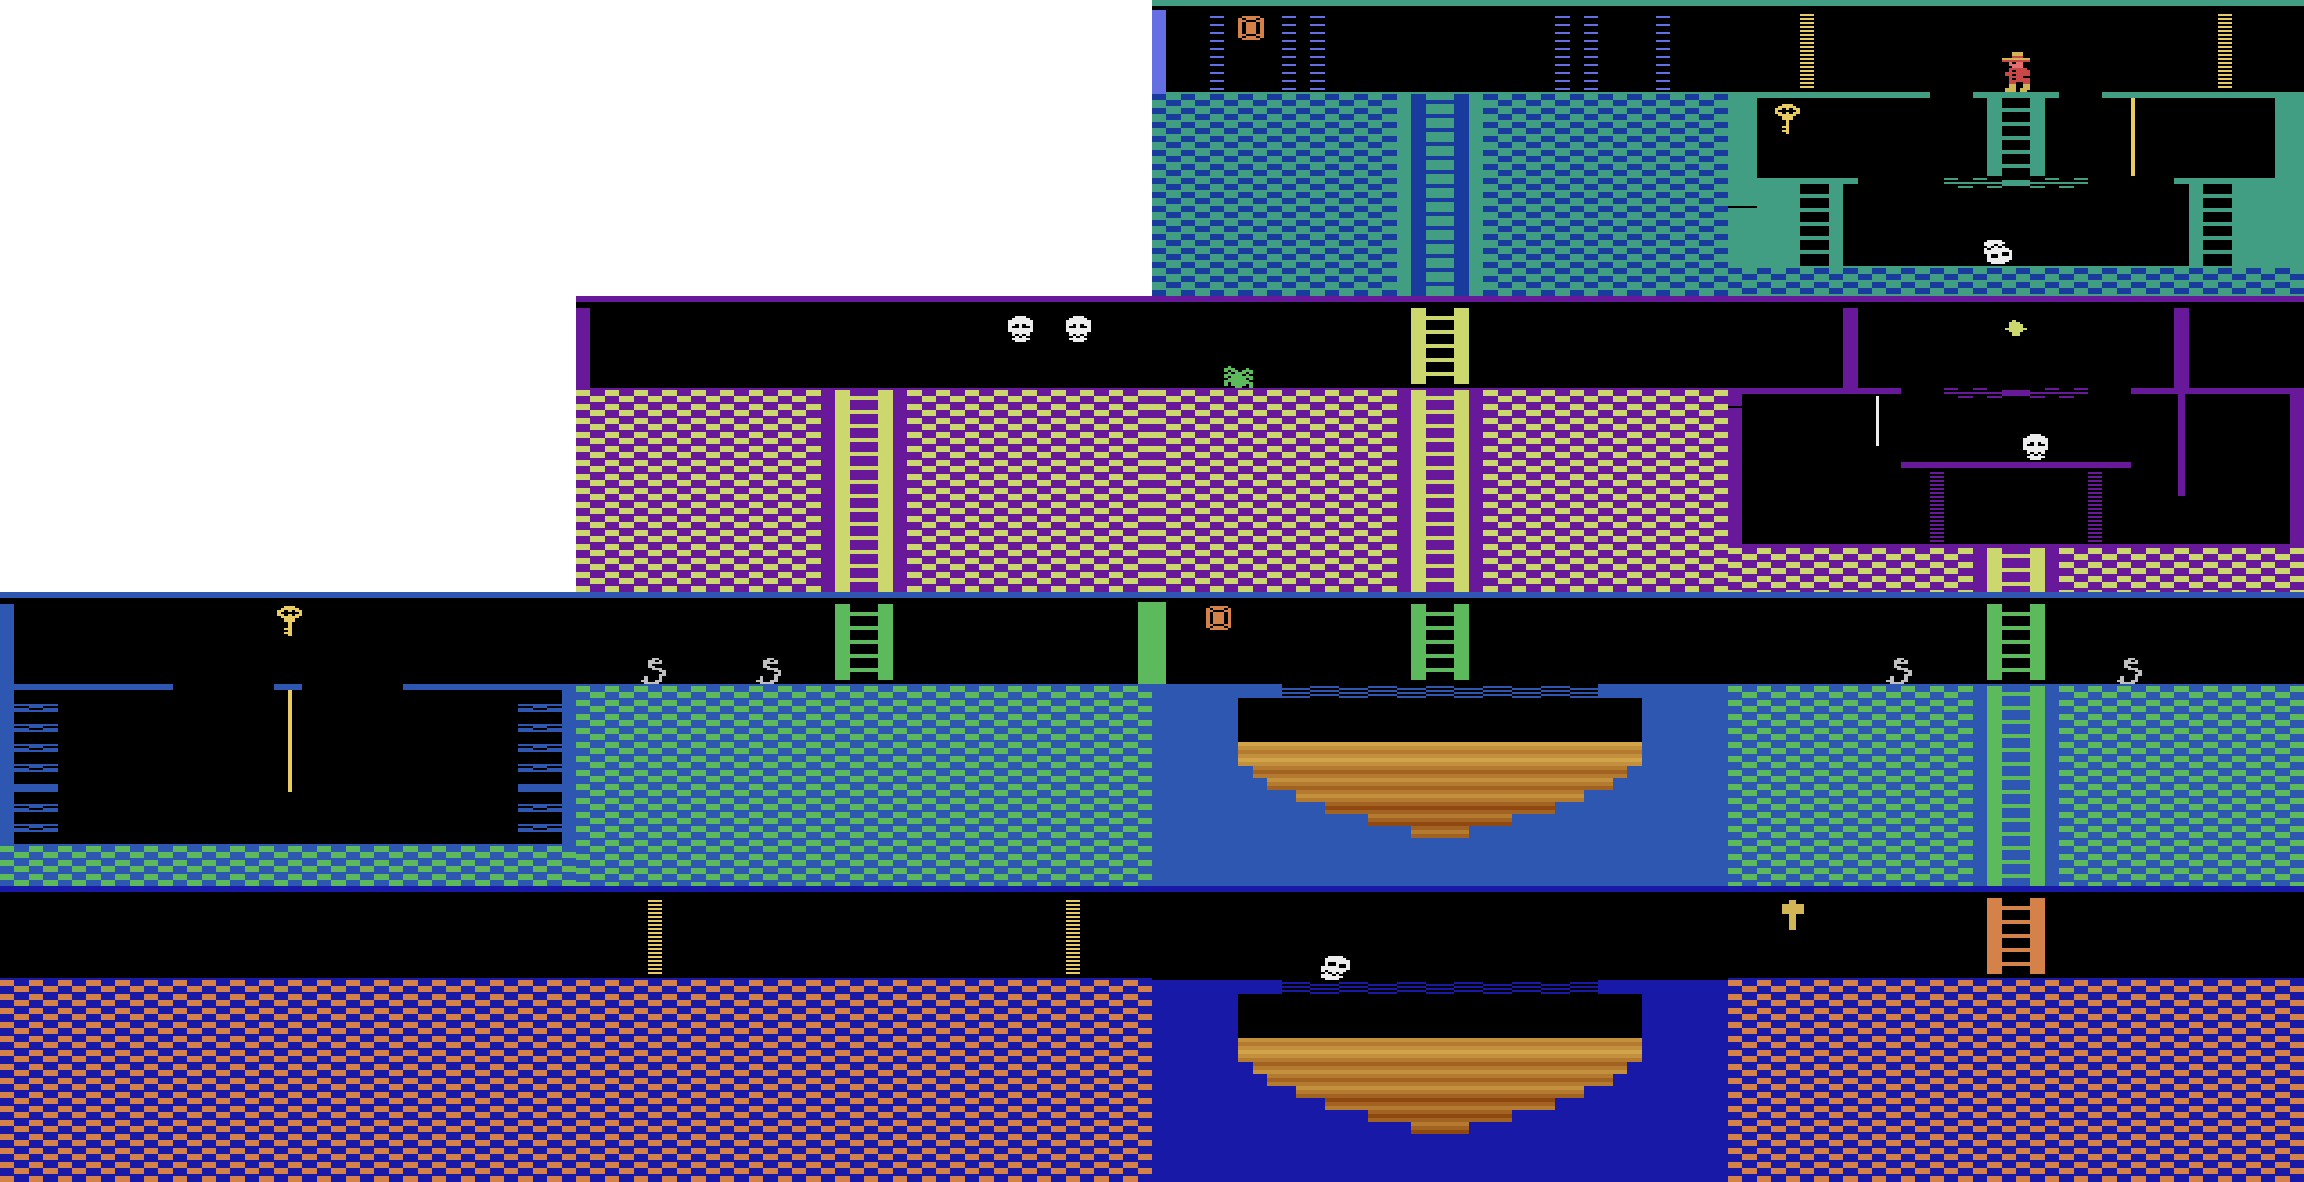
\includegraphics[width=\unitlength]{img/montezuma_all_pt1.png}}
    \put(.58,.485){\color[rgb]{1,1,1}\makebox(0,0)[lb]{0}}
    \put(.83,.485){\color[rgb]{1,1,1}\makebox(0,0)[lb]{1}}
    \put(.33,.357){\color[rgb]{1,1,1}\makebox(0,0)[lb]{3}}
    \put(.58,.357){\color[rgb]{1,1,1}\makebox(0,0)[lb]{4}}
    \put(.83,.357){\color[rgb]{1,1,1}\makebox(0,0)[lb]{5}}
    \put(.08,.228){\color[rgb]{1,1,1}\makebox(0,0)[lb]{8}}
    \put(.30,.228){\color[rgb]{1,1,1}\makebox(0,0)[lb]{9}}
    \put(.58,.228){\color[rgb]{1,1,1}\makebox(0,0)[lb]{10}}
    \put(.83,.228){\color[rgb]{1,1,1}\makebox(0,0)[lb]{11}}
    \put(.08,.1){\color[rgb]{1,1,1}\makebox(0,0)[lb]{16}}
    \put(.33,.1){\color[rgb]{1,1,1}\makebox(0,0)[lb]{17}}
    \put(.6,.1){\color[rgb]{1,1,1}\makebox(0,0)[lb]{18}}
    \put(.83,.1){\color[rgb]{1,1,1}\makebox(0,0)[lb]{19}}
  \end{picture}
%}

\vspace{.2cm}

%\noindent\makebox[\textwidth]{
  \begin{picture}(1,.513)
    \put(0,0){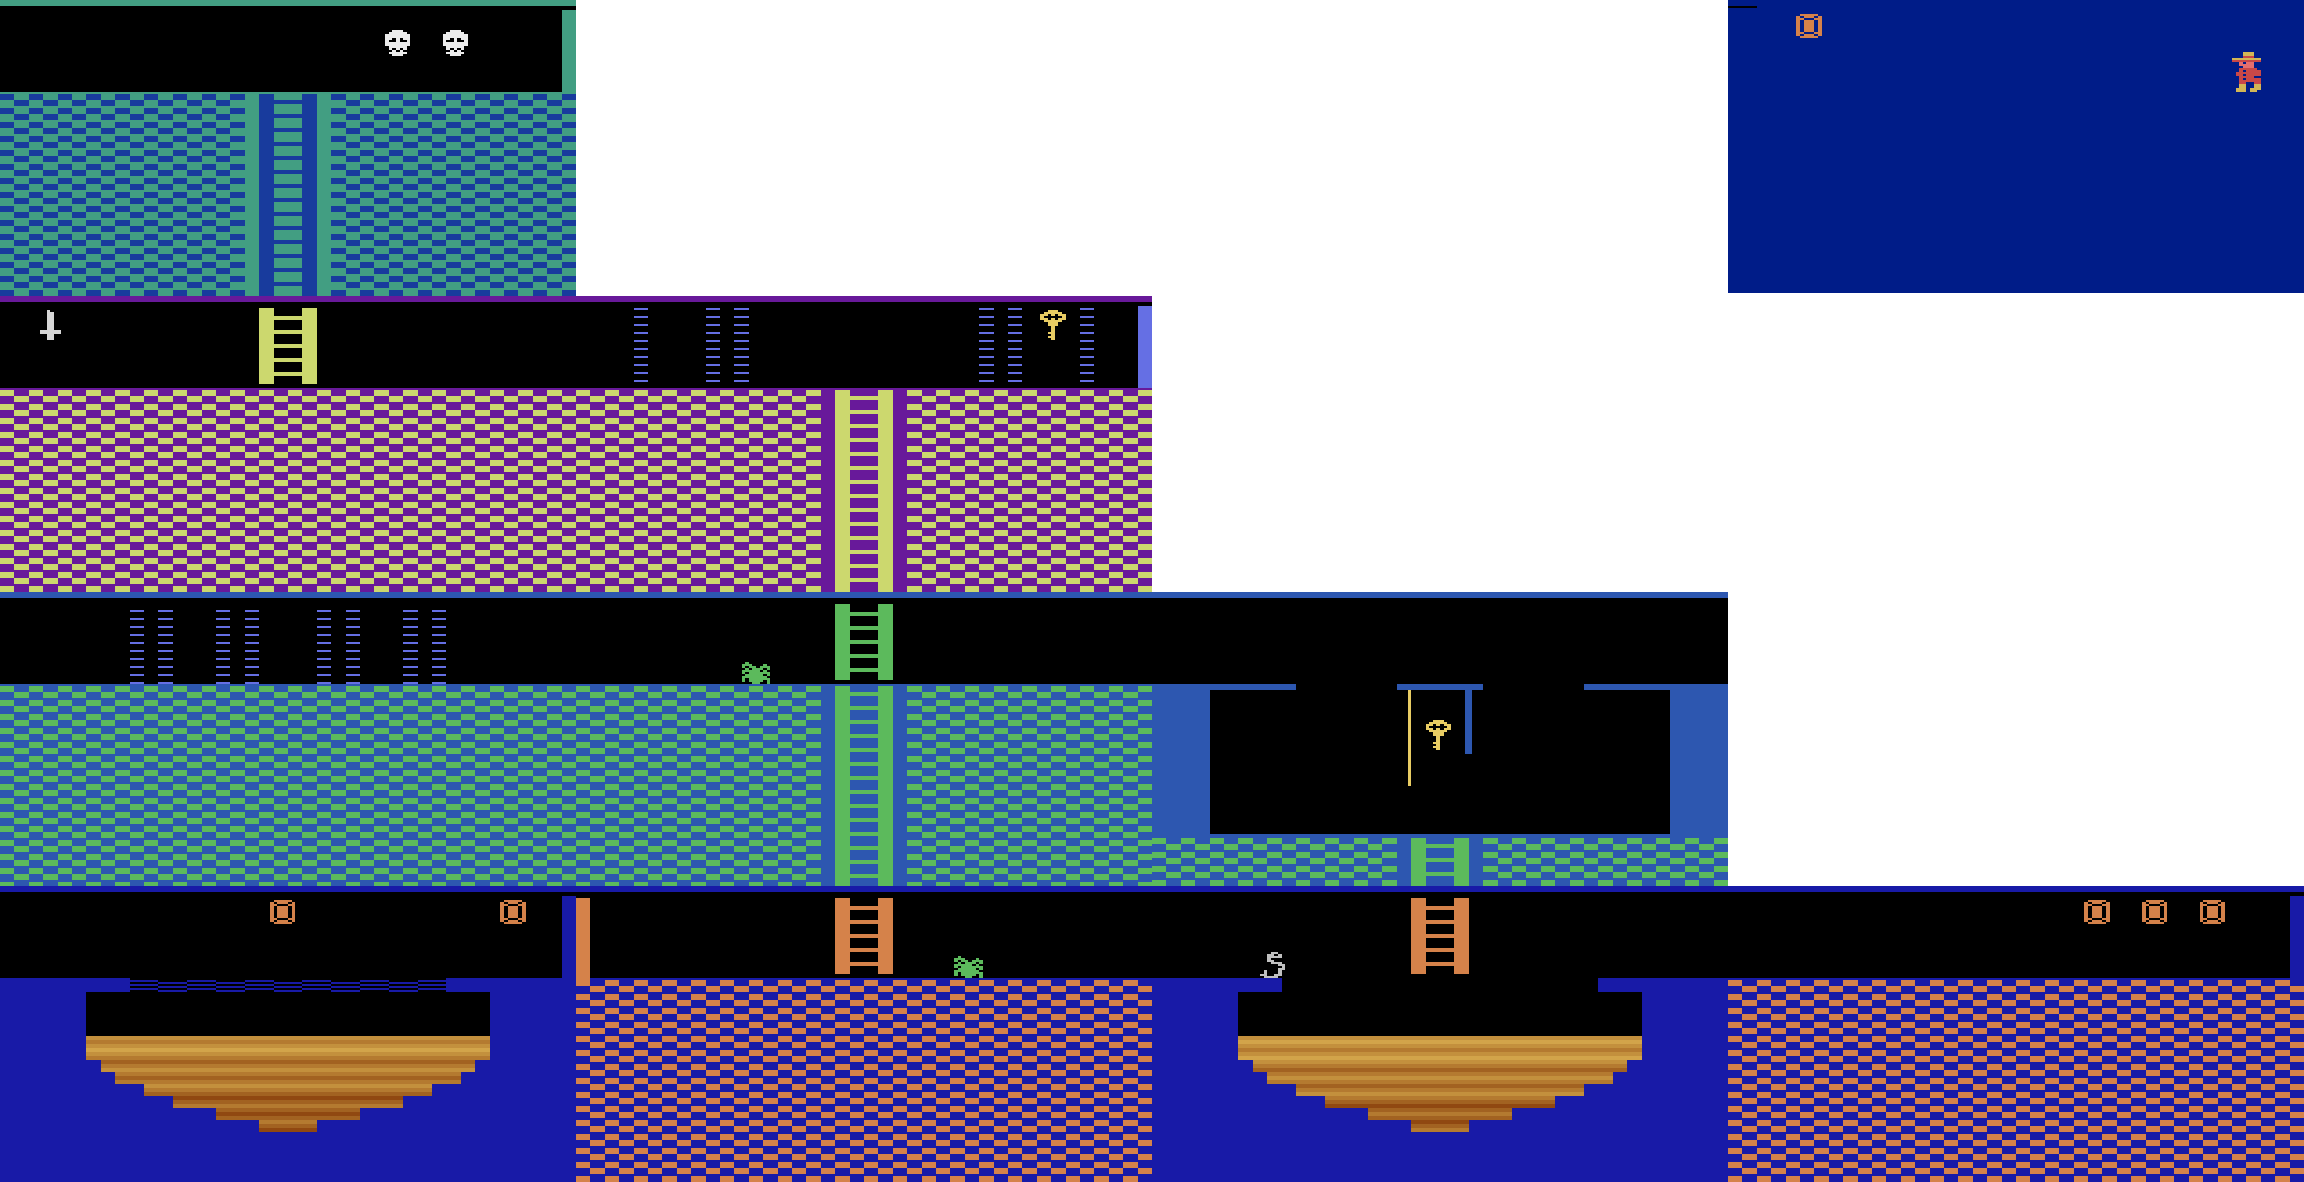
\includegraphics[width=\unitlength]{img/montezuma_all_pt2.png}}
    \put(.08,.485){\color[rgb]{1,1,1}\makebox(0,0)[lb]{2}}
    \put(.83,.485){\color[rgb]{1,1,1}\makebox(0,0)[lb]{15}}
    \put(.08,.357){\color[rgb]{1,1,1}\makebox(0,0)[lb]{6}}
    \put(.33,.357){\color[rgb]{1,1,1}\makebox(0,0)[lb]{7}}
    \put(.04,.228){\color[rgb]{1,1,1}\makebox(0,0)[lb]{12}}
    \put(.28,.228){\color[rgb]{1,1,1}\makebox(0,0)[lb]{13}}
    \put(.58,.228){\color[rgb]{1,1,1}\makebox(0,0)[lb]{14}}
    \put(.08,.1){\color[rgb]{1,1,1}\makebox(0,0)[lb]{20}}
    \put(.33,.1){\color[rgb]{1,1,1}\makebox(0,0)[lb]{21}}
    \put(.58,.1){\color[rgb]{1,1,1}\makebox(0,0)[lb]{22}}
    \put(.83,.1){\color[rgb]{1,1,1}\makebox(0,0)[lb]{23}}
  \end{picture}
%}
\end{center}
\caption[The complete map of \acl{MR}.]{The complete map of \acl{MR}. Rooms are
numbered from left to right and from top to bottom. The pyramid they form has
been cut to fit in the page. Room 15 is located to the left of room 16. The
screens are not numbered in the game. The player starts in room 1 and finishes
in room 15.\label{fig:montezuma-map}}
\end{figure}

\subsection{Reverse-engineering \acl{MR}}
We used the \acl{ALE} (\cite{bellemare2013arcade}) to take several simultaneous
screen and \ac{RAM} snapshots. We usually took 5 to 10 snapshots in the space of
1 or 2 seconds, while performing certain action in the game. Then, we looked at
the bytes that changed value from snapshot to snapshot.

We also used the debugger built-in to the Atari 2600 emulator, Stella
(\cite{stella}). Using the command \verb-breakif <condition>-, that pauses the
game and shows the debugger if a condition is met, enabled us to play and check
whether a memory position behaved as we suspected. In some cases we used the
disassembled code in that debugger too.

In \ffref{tab:atari-ram} and in the list below we reproduce the layout of
the Atari 2600's main memory and what each position affects in \acl{MR}.

Some entries can be modified in the Stella debugger when the game is running,
and affect the game. If an entry is not editable, it will be marked with an
asterisk (*). The values that are not marked editable may be editable in other
circumstances, and are probably editable in the middle of the computations
within a frame. However, their value has been observed only going back to what
it was if modified between frames.

\fxwarning{Explain the Atari's RAM, explain Panama Joe}
\fxwarning{Talk about the RAM of the Atari having 128 bytes and the ones
  relevant are 0x80 0xff. Also about the ROM}
\fxwarning{TAlk about MR.
There seem to be two sprites drawn to screen: one "key" and one "skull", named
after them in the first screen. We will call the first "collectible sprite", but
it can be a monster too}


\begin{table}[hbtp]
\begin{center}
\newcommand{\ram}[2]{\hyperref[ram:#1]{#2*}}
\newcommand{\rame}[2]{\hyperref[ram:#1]{#2}}
%\newcommand{\ram}[2]{\ref{ram:#1}*}
%\newcommand{\rame}[2]{\ref{ram:#1}}
\begin{tabular}{c|cccccccccccccccc}
  & 0 & 1 & 2 & 3 & 4 & 5 & 6 & 7 & 8 & 9 & A & B & C & D & E & F \\
\hline
8 &   &   &   &\rame{screen}{83}&   &   &   &   &   &   &   &   &   &   &   &   \\
9 &   &   &   &\rame{score}{93}& \rame{score}{94}& \rame{score}{95}&   &   &   &   &   &   &   &   &\ram{player-sprite}{9E}&   \\
A &   &   &   &   &   &   &   &   &   &   &\rame{x}{AA}&\rame{y}{AB}&   &   &   &   \\
B &   &\rame{collectable}{B1}&\rame{collectable-colour}{B2}&  &\rame{look-lr}{B4}&  &   &   &   &   &   \rame{lives}{BA} & & & &\rame{skull-animation}{BE}&\rame{skull-jump-y}{BF}\\
C &   &\rame{inventory}{C1}&\ram{doors}{C2}&\rame{skull-moving}{C3}&   &   &   &   &   &   &   &   &   &   &\rame{skull-rotate-y}{AE}&\rame{skull-rotate-x}{AF}\\
D &   &   &   &   &\rame{sprite-modifier}{D4}&   &  \rame{jump}{D6}&   &\rame{fall}{D8}&   &   &   &   &   &  & \\
E &   &   &   &   &   &   &   &   &   &   &\ram{skull-n-rotations}{EA}&   &   &   &   &   \\
F &   &   &   &   &   &   &   &   &   &   &   &   &   &   &   &   \\
\end{tabular}

\end{center}
\caption{The known \acs{RAM} layout for \acl{MR}.\label{tab:atari-ram}}
\end{table}

{
\newcommand{\entry}[2]{\item\label{ram:#1}\textbf{0x#2}: Not editable.}
\newcommand{\entrye}[2]{\item\label{ram:#1}\textbf{0x#2}: Editable.}
\newcommand{\n}[1]{0x#1}

\begin{enumerate}
\entrye{lives}{BA} The number of lives the player has left, that is, the number of
times the player can die and continue the game afterwards. Controls the number
of hats displayed at the top. Panama Joe starts with 5 lives. The counter can go
up to 6 without graphical problems.

\entrye{screen}{83} The current screen. If edited, the new screen will only be
partially drawn. Sometimes, one can exit the screen and reenter it by playing
and the issue will go away.

\entrye{x}{AA} The X position of the character. If set to the middle of the air,
Panama Joe will fall.

\entrye{y}{AB} The Y position of the character. If set to the middle of the air,
and there is a platform below, the character will not fall! Instead, it will
behave as if it was on a ladder. The Y values of the three floors that every
level has are \n{94} or \n{9C}, \n{C0}, and \n{EB}.

\entrye{jump}{D6} The current frame of the jump. Set to \n{FF} when in the
ground. Set to \n{13} when the jump starts. When jumping, the game adds to the Y
of Panama Joe the values from the array starting at memory position \n{E47}.
Thus, if set to higher than \n{13}, the game behaves oddly. It also can be reset
to whatever value at any time, causing Panama Joe to start a jump, even in
mid-air.

\entrye{fall}{D8} The current frame of the fall. Normally set to \n{00}. When falling
off an elevated ground, or off a jump, this value will begin to count up. If it
is \n{08} or higher when Panama Joe touches the ground, he will die.

\item\label{ram:score}\textbf{0x93}, \textbf{0x94}, \textbf{0x95}: Editable. The
score, represented in \acl{BCD}. This is, every nibble represents a decimal digit.

\entrye{inventory}{C1} The contents of the player's inventory. Each possible
object in it is associated to a bit, that is set if the object is in the
inventory. At most 6 objects can be carried without causing graphical
corruptions. The objects and their associations are:
\begin{center}
\begin{tabular}{c|c|c|c|c|c|c|c}
\n{80} & \n{40} & \n{20} & \n{10} & \n{08} & \n{04} & \n{02} & \n{01} \\
\hline
torch & sword & sword & key & key & key & key & mallet \\
\end{tabular}
\end{center}
If the inventory's value is changed, collecting items the normal way stops
working.

\entry{doors}{C2 (bits 3, 2)} Whether the doors in the screen are closed or
open. Only means this in screens 1, 5 and 17. When the bit is set, the door is
closed. Bit 3 controls the door in the left, bit 2 the one in the right.

\entrye{skull-animation}{BE} The frame of the rotating skull's animation, in
screens where there is one.

\entrye{skull-rotate-x}{AF} X of the rotating skull, when there is one (screens
1 and 18). It is not in the same scale as the player's X.
\entrye{skull-rotate-y}{AE} Y of the rotating skull. Also in its own scale, and
cannot take it away from its floor.

\entry{skull-n-rotations}{EA} The number of times the rotating skull in the
first screen has changed direction. Remains even after changing screen. If
untouched, the lowest byte indicates the direction the skull is moving in. Can
be changed, but it does not change the direction of the skull.

\entrye{skull-jump-y}{BF} relative Y position of the jumping skulls, in screens where they are present.
It oscillates between \n{00} and \n{0F}, where 0 is the topmost position. The
game makes relative changes to this value, so if set to F while the skulls on
mid-air, they will not go below that point afterwards.

\entrye{skull-moving}{C3 (bit 1)} Whether the rotating skull is moving (set) or
not (unset). The function of the rest is unknown.

\entry{player-sprite}{9E} The current sprite drawn for Panama Joe. This is what
changes every few frames to show the character moving. Possible values: (\n{00})
standing still, (\n{2A}) walking frame, (\n{3E}) still, on a ladder, (\n{52})
ladder climbing frame (\n{7B}) still, on a rope, (\n{90}) climbing a rope,
(\n{A5}) mid-air, (\n{BA}) upside down, left foot up, (\n{C9}) upside down,
right foot up, (\n{DD}, \n{C8}) alternate flashing frames when dead by a monster.

\entrye{look-lr}{B4 (bit 3)} Whether Joe is looking to the left (set) or the
right (unset). The function of the rest is unknown.

\entrye{collectable}{B1} The collectable sprite that is drawn. Each screen has
an associated position where a sprite that may be collected, or a monster, is
drawn. The things that are drawn, associated with the value of the byte that
draws them, are: (0) no sprite, (1) jewel, (2) sword, (3) mallet, (3) key, (5) jumping
skeleton, (6) torch, (7) blinking snake-torch, (8) snake, (9) blinking
snake-spider, (A) walking spider. The rest of the values cause corruption. The
colour of this sprite is controlled by memory position
\hyperref[ram:collectable-colour]{\n{B2}}.

\entrye{collectable-colour}{B2} The colour of the collectable sprite. All values
of the byte seem produce a valid colour and no corruption.

\entrye{sprite-modifier}{D4} Modifies collectables (from
\hyperref[ram:collectable]{\n{B1}}), monsters and ropes. The values and their
effects are: (0) one sprite, (1) two sprites, (2) two sprites, separated with enough
space for another sprite, (3) three sprites, filling the space in value 2, (4)
two sprites, very separated, (5) the sprites become wide, (6) three very
separated sprites, (7) a very wide sprite. Only the three least significant bits
seem to affect anything.

\end{enumerate}
}

\subsection{Reward shaping\label{subsec:reward-shaping}}
\begin{figure}[hbtp]
\begin{center}
\noindent\makebox[\textwidth]{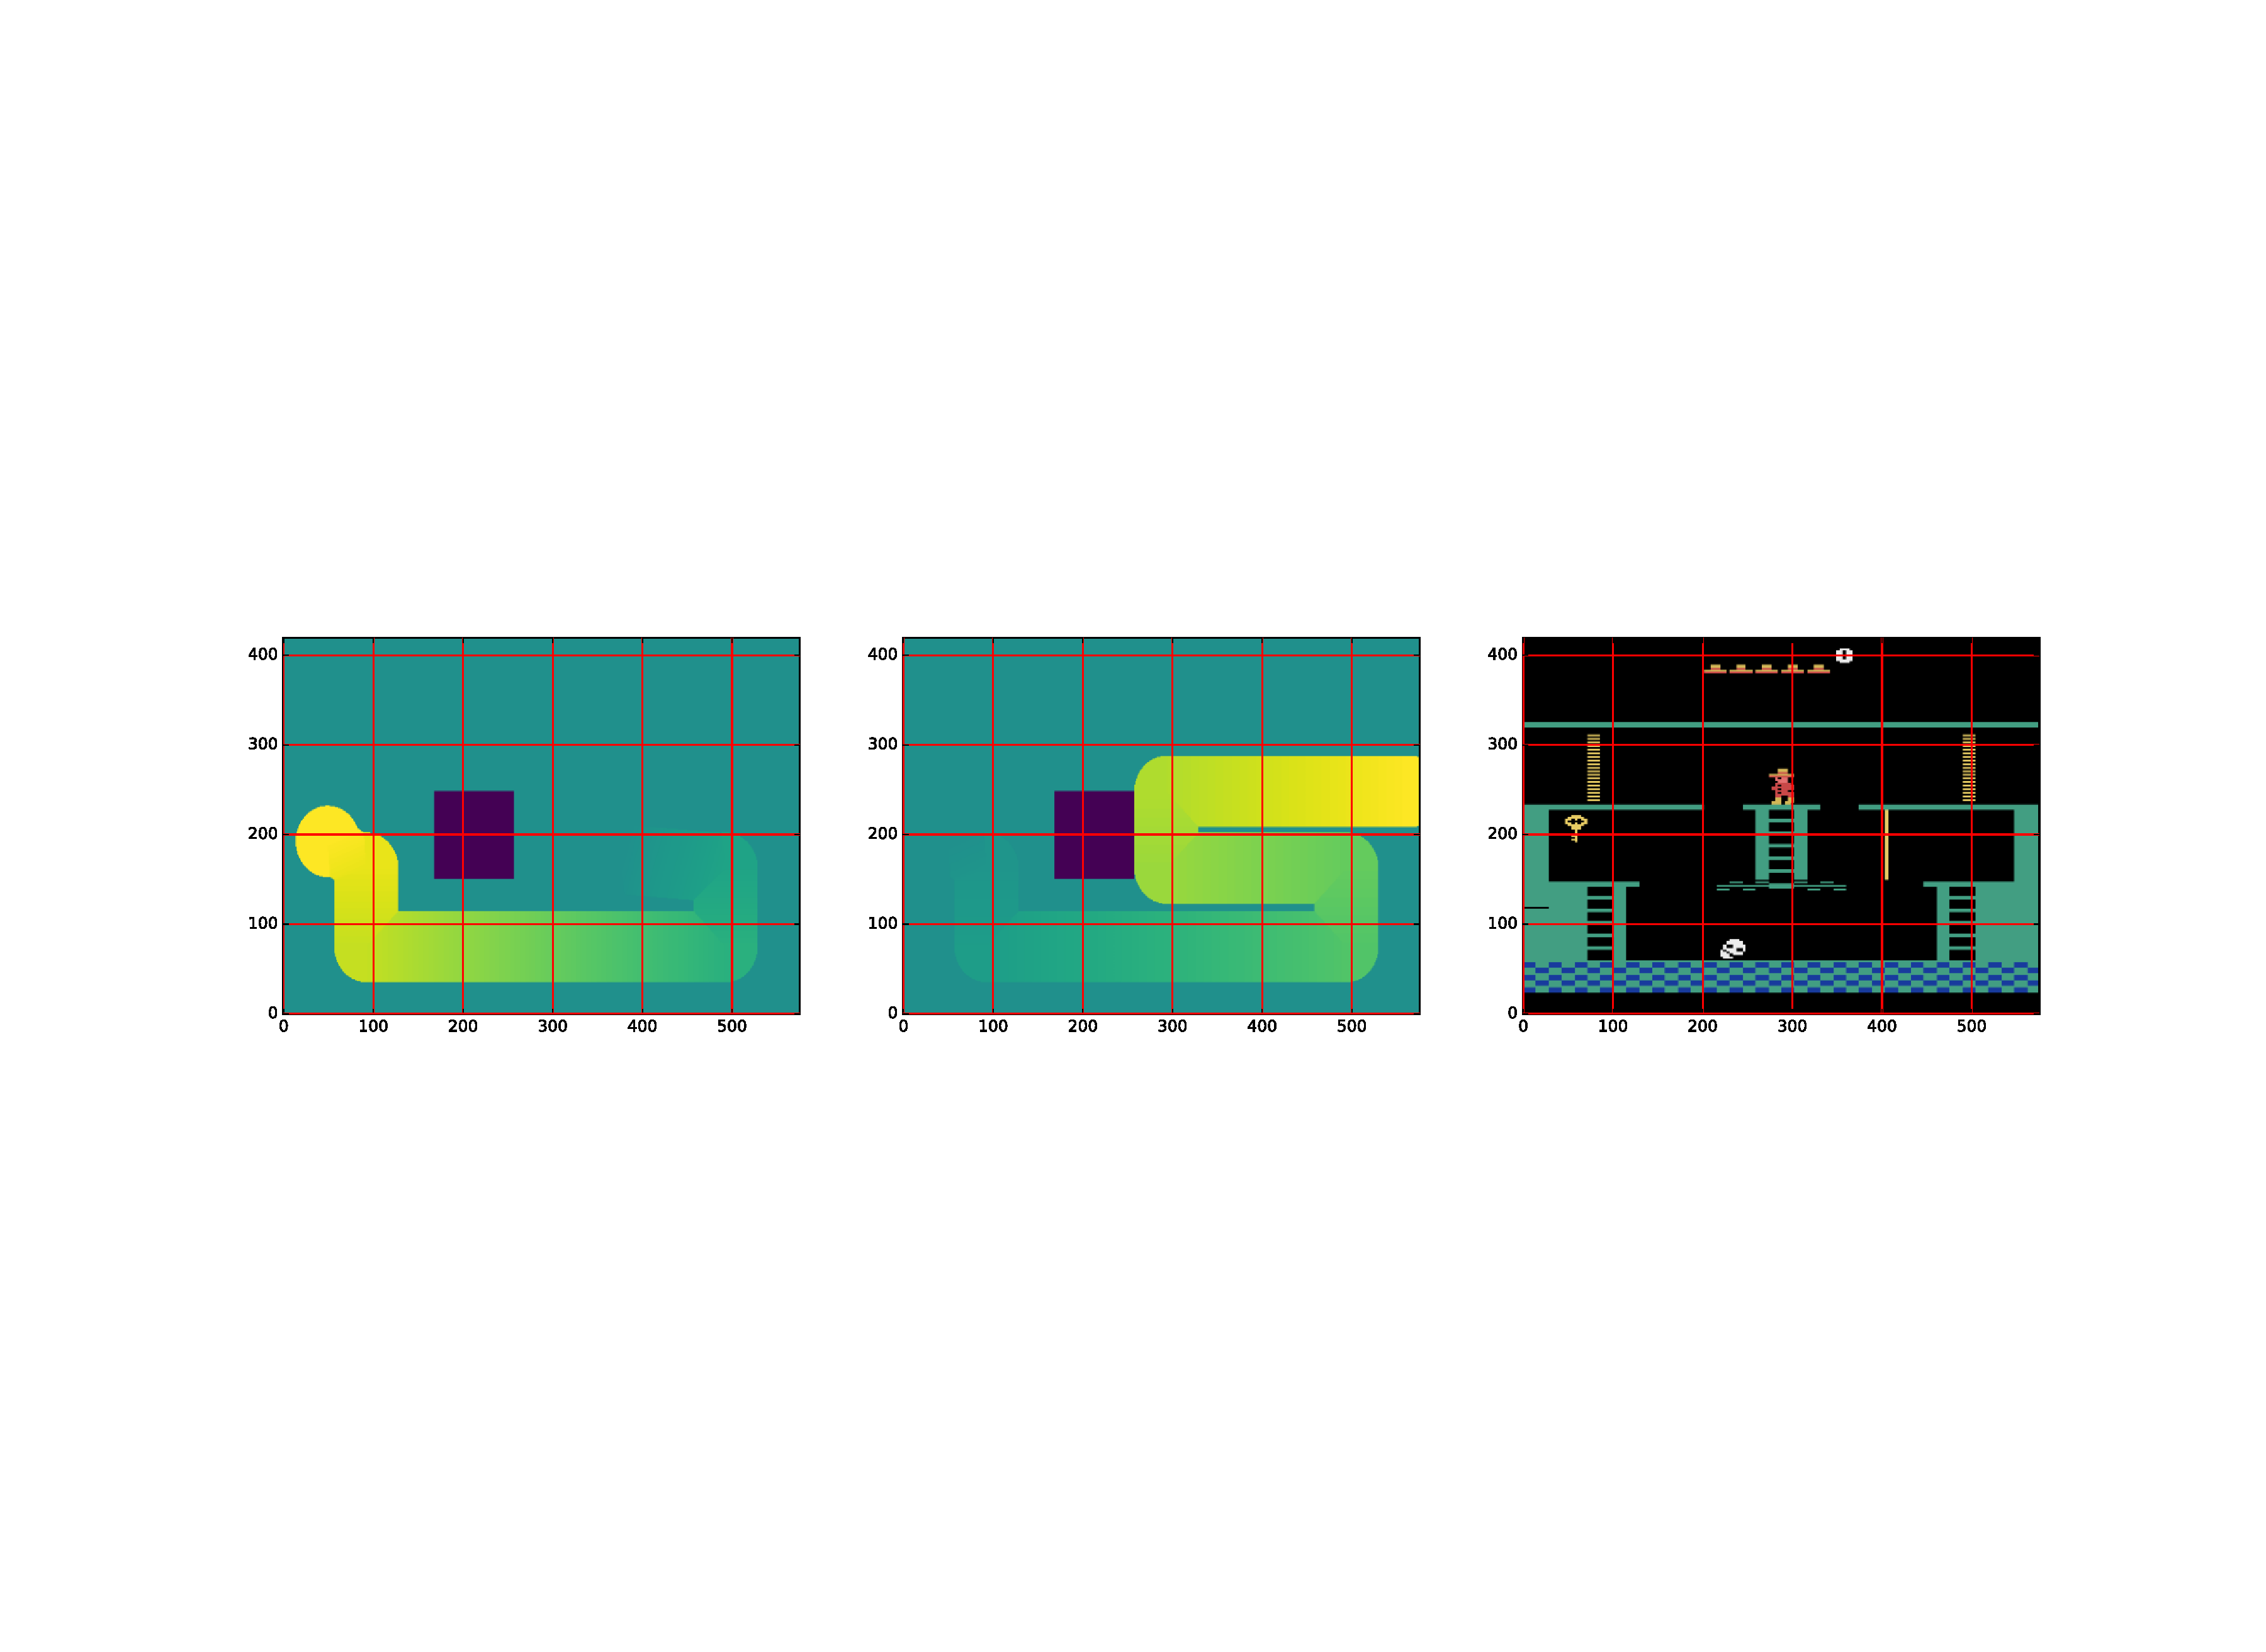
\includegraphics[width=\paperwidth - 1in]{img/shaping.pdf}}
\end{center}
\caption{The shaping potential field used, before and after grabbing the
key.\label{fig:shaping}}
\end{figure}
\begin{equation}
  t_1 = \frac{v_{x_2}(y_1-y_2) - v_{y_2}(x_1-x_2)}{v_{y_2}v_{x_1} - v_{x_2}v_{y_1}}
\end{equation}
\section{Planning}
\subsection{\acl{IW}(1)}
\subsection{\acl{IW}(3) on location}
\subsection{\acl{IW}(3) on location with heuristic}
\section{Learning}
\subsection{Shaped tabular Sarsa}
\subsection{Task by task \acs{DQN}}
\subsection{Tabular Sarsa combined with planning}

%%% Local Variables: 
%%% mode: latex
%%% TeX-master: "../report"
%%% End: 
\cleardoublepage
\chapter{Evaluation}
\section{Planning\label{sec:score-planning}}
We evaluated the domain-specific planning algorithm described in
\ffref{alg:iw-optimised}, with different subsets of enhancements and different
parameters. We used the \ac{ALE}, with deterministic games
(\verb-repeat_action_probability=0-). Our code is based in the one available
from \citet{lipovetzky2015classical}.

Recall that our \ac{IW}(3) only evaluates position for pruning, not
on any other tuple.

\begin{itemize}
  \item $max_{ef}$: maximum nodes emulated per frame.
  \item $\gamma$: The discount factor.
  \item $n_a$: number of actions to take without re-planning.
  \item $p_r$: probability that a room is pruned. Blank means zero.
  \item \textit{FS}: frame skip, the amount of frames each action is taken for.
  \item \textit{TR}: Whether the search tree is reused, or the nodes are
    re-emulated in every frame.
  \item Frontier: the data structure/s used to store the frontier:
    \begin{itemize}
      \item $q$: a single \ac{FIFO} queue, like \ac{BFS} and \ac{IW}.
      \item $q,q_l$: two \ac{FIFO} queues, one with a lower priority.
      \item P. Dist.: Priority queue that prioritises nodes more distant (in
        game coordinates, Euclidean distance) to the root.
      \item 2BFS Two priority queues: one prioritising low novelty, breaking
        turns by largest accumulated return, and one prioritising large
accumulated return, breaking ties by lowest novelty \citep{lipovetzky2015classical}.
    \end{itemize}
    \ac{FIFO} queue, 2 \ac{FIFO} queues, or a priority queue.
  \item \textit{EB}: Exploration Bonus. Whether the agent gains 1 reward on
    exploring a new screen.
  \item \textit{OAV}: Obstacle Algorithm Version. The algorithm that waits for
    obstacles to disappear has some variants. Blank means the absence of such
    thing. Version 1 is the nodes that lead into an obstacle are re-enqueued in
    the frontier. Versions between 1 and 2 are other semi-successful
    modifications of it. Version 2 is the one explained in
Subsections~\ref{subsec:domain-explanation} and~\ref{subsec:implementation-iw}.
  \item \textit{EA}: Extended Action set. Whether the algorithm uses the 18
actions possible with the Atari or the 8 distinct actions in \ac{MR}.
\end{itemize}

Additionally, algorithms with an asterisk (*) receive negative rewards (-5000)
on death. The remaining parameters' values are: $max\_wait=20$, $max\_backtrack=7$.

\begin{table}[hbtp]
  \begin{center}
  \begin{tabular}{c|ccccccccccc|c}
    Name       & $max_{ef}$ & $\gamma$ & $n_a$ & $p_r$ & FS & TR         & Frontier & EB         & OAV & EA         & Score     \\
\hline
    \ac{IW}(1) & 150k       & 0.995    & 1     &       & 5  & \checkmark & $q$      &            &     & \checkmark & 0         \\
    2BFS       & 150k       & 0.995    & 1     &       & 5  & \checkmark & 2BFS     &            &     & \checkmark & 540       \\
    \ac{IW}(3)*  & 150k       & 0.995    & 1     &       & 5  &            & $q$      &            &     &            & 4600      \\
    \ac{IW}(3)*  & $1\,500$k  & 0.995    & 1     &       & 5  &            & P. Dist. &            & 1   &            & $2\,500$  \\
    \ac{IW}(3)*  & 300k       & 0.995    & 1     &       & 5  &            & $q,q_l$  & \checkmark & 1   &            & $5\,600$  \\
  \hline
    \ac{IW}(3)*  & 300k       & 0.995    & 1     &       & 5  &            & $q,q_l$  & \checkmark & 1.1 &            & $8\,000$  \\
    \ac{IW}(3)*  & 150k       & 0.99     & 1     &       & 10 &            & $q,q_l$  & \checkmark & 1.1 &            & $10\,200$ \\
    \ac{IW}(3)*  & 75k        & 0.985    & 1     &       & 10 &            & $q,q_l$  & \checkmark & 1.1 &            & 0         \\
    \ac{IW}(3)*  & 10k        & 0.98     & 1     &       & 20 &            & $q,q_l$  & \checkmark & 1.1 &            & 0         \\
  \hline
    \ac{IW}(3)   & 300k       & 0.995    & 1     &       & 6  &            & $q,q_l$  &            & 1.2 &            & 100       \\
    \ac{IW}(3)   & 300k       & 0.999    & 1     &       & 5  &            & $q,q_l$  &            & 1.2 &            & 500       \\
    \ac{IW}(3)   & 300k       & 0.995    & 1     &       & 5  &            & $q,q_l$  &            & 1.2 &            & $6\,700$  \\
    \ac{IW}(3)   & 300k       & 0.999    & 1     &       & 5  &            & $q,q_l$  & \checkmark & 1.2 &            & $7\,100$  \\
  \hline
    \ac{IW}(3)   & 300k       & 0.999    & 1     & 0.25  & 5  &            & $q,q_l$  & \checkmark & 1.2 &            & $4\,700$  \\
    \ac{IW}(3)   & 300k       & 0.99     & 1     & 0.2   & 5  &            & $q,q_l$  & \checkmark & 1.2 &            & $11\,000$ \\
  \hline
    \ac{IW}(3)   & 300k       & 0.99     & 1     & 0.2   & 5  &            & $q,q_l$  & \checkmark & 2   &            & $13\,600$ \\
    \ac{IW}(3)   & 150k       & 0.99     & 2     & 0.2   & 10 & \checkmark & $q,q_l$  & \checkmark & 2   &            & $14\,500$ \\
    \ac{IW}(3)   & 150k       & 0.995    & 2     & 0.2   & 5  & \checkmark & $q,q_l$  &            & 2   &            & $8\,000$  \\
    \ac{IW}(3)   & 150k       & 0.995    & 2     & 0.2   & 5  & \checkmark & $q,q_l$  & \checkmark & 2   & \checkmark & $7\,800$  \\
    \ac{IW}(3)   & 150k       & 0.999    & 3     & 0.2   & 5  & \checkmark & $q,q_l$  & \checkmark & 2   &            & $14\,900$ \\
\end{tabular}
\end{center}
\caption{The results of different planning algorithm variations}
\end{table}

The algorithm described in \ffref{subsec:domain-explanation} obtains the same
score as the latest one, but it avoids opening the two doors. Instead, it finds
a glitch in the game that allows it to spend the two keys without a door. A video of it is available
\href{https://www.youtube.com/watch?v=KSPYzLE0uy8}{online}. The glitch happens
around \href{https://youtu.be/KSPYzLE0uy8?t=172}{2:52}.

To obtain this massive increase in score, we have heavily tweaked the algorithm to this
game. The strategies employed will likely not generalise to all classes of
problems. Some of them might be useful for games that happen in a 2D
spatial environment, such as pruning on position, waiting for obstacles. The
random room pruning heuristic may also be useful in other problems in the
on-line setting that demand exploring multitudes of similar paths.

%IW(1) geffner
%
%no tree reuse, no exploration bonus
%IW(3) with a big negative reward when dying:  8 screens, 4600 score
%
%IW(3) with no incentives and a priority queue prioritising nodes farther away
%2500 score
%
%IW(3) big negative, with double queue, 9 screens 5600 score
%.995, 30000, sscore 5600
%^ with exploration bonus
%
%exploration bonus:
%
%big negative too
%IW(3) re-enqueuing nodes that run into an obstacle 8000, 300k nodes/frame
%same but .99 discount and 10 frame actions 150k nodes/frame: 10200
%sambe but 15, .985, 10k n/f, 0
%same but 20 , 75k nodes and .98 discount 0
%
%
%Ancestors:
%
%No exploration bonus, no death avoidance
%6 frameskip, .995 -> 100 score
%5 frameskip, .999 -> 500
%5 frameskip, .995 -> 6700
%
%with exploration bonus, .999 -> 7100 score
%
%More than 1 action per frame:
%7500 reward
%
%
%Moreexplore
%no incentives: 2900, incentives 8000
%with 10 and .995: 2500, 2900
%
%noreopen: with screen prune probability
%0.25:, discount .999 : 4700
%.2, discount .99 : 13600 (11015 with old algo)
%
%fs 10, actions no recalc 2: 14500 incentives
%
%no explore but with the good pruning, 2 actions, and teh good navigation :8000
%
%with explore but with 18 actions: 7800
%%
%.999 discount
%14900: good exploration with exploration incentives, calc every 3 actions
%(avoids taking a wrong path)
%

\section{Learning}
We trained agents on the first screen of \acl{MR} using the Sarsa algorithm,
with and without options, and using our shaping function
(\ffref{subsec:shaping-function}).

We used a learning rate $\alpha=0.01$ and a discount rate $\gamma=0.995$. We
also used the \emph{annealing} training technique, which consists in reducing
the $\varepsilon$ for the $\varepsilon$-greedy strategy every episode. When
training without annealing we used $\varepsilon=0.1$, and when training with
annealing we used $\varepsilon=\textsc{Max}(0.7 - 3\cdot 10^{-5} \cdot n_e,
0.1)$, where $n_e$ is the episode number. This encourages extra exploration at
the beginning.

The average reward over time can be seen in Figures \ref{fig:q-noopts-noanneal},
\ref{fig:q-noopts-anneal}, \ref{fig:q-opts-noanneal} and
\ref{fig:q-opts-anneal}. In each of those figures, at the left the reward
including the shaping reward is shown, and at the right the environment reward
alone is shown.

\newcommand{\drawtraining}[2]{
\begin{figure}[hbtp]
\begin{center}
\includegraphics[width=\textwidth/2- 0.2cm]{img/#1-phi.pdf}
\includegraphics[width=\textwidth/2- 0.2cm]{img/#1.pdf}
\end{center}
\caption{#2\label{fig:#1}}
\end{figure}
}

\drawtraining{q-noopts-noanneal}{The reward over time, without options or
annealing. $y$ axis is reward, $x$ axis is thousands of episodes.}
\drawtraining{q-noopts-anneal}{The reward over time, without options, with
annealing. $y$ axis is reward, $x$ axis is thousands of episodes.}
\drawtraining{q-opts-noanneal}{The reward over time, with options but without
annealing. $y$ axis is reward, $x$ axis is thousands of episodes.}
\drawtraining{q-opts-anneal}{The reward over time, with options and with
annealing. $y$ axis is reward, $x$ axis is thousands of episodes.}

There is something odd about all the graphs. First, both graphs that do not use
options (Figures \ref{fig:q-noopts-noanneal} and \ref{fig:q-noopts-anneal}),
actually \emph{decrease} in accumulated reward during the first $\sim 25\,000$
episodes. However, the accumulated reward without accounting for the shaping
function is almost monotonically increasing. We suspect that the return in the
starting state is also monotonically increasing, and it is the unique form of
the shaping function $F(s, a, s') = \gamma\phi(s') - \phi(s)$ that permits this
to happen.

It is also somewhat worthy of note that the annealed version takes longer start
increasing in reward, but once it does it converges earlier. We attribute this
to an early exploration of ``accidental'' states that makes the agent learn them
thoroughly at first, and then make it have no problems when spuriously
encountering them afterwards.

As for the versions with options, they do not work at all. Videos of
the agent acting show that it learns to jump to the left, dying as fast as
possible. The reward it gains in doing so is negative, and less than it gains if
it jumps to the right and follows with the plan as the agents without options,
but the options do not seem to fit.
  
%Show the shaping that we did and the learning curve, compare with old shaping
%using options, compare with shaping using options, show reward without shaping.

%If a deterministic policy is taken, the reward is always 4. A video of that 

%%%%%%%%%%%%%%%%%
% Last line of the epochs is possibly a bug, it evaluated rewards.txt
%%%%%%%%%%%%%%%%%

%both noanneal and montezuma phi options are monzteaumz options!! The most
%recent is noanneal.
% first cont_phi is phi_regular_2016_06_17_15_37_03
% second cont_phi is phi_noanneal_2016_06_17_15_36_51
\subsection{The pitfalls of shaping\label{subsec:evaluation-shaping}}
Prior to reading about shaping functions that do not vary the optimal policy, we
tried to lay down a path of ``pellets'' that the agent would get reward for
collecting, from the start to the key. We arranged them in a line, and made it
so that collecting one pellet also collected all the previous ones. We tried to
mitigate this by reducing the number of pellets the agent could get at once, but
then it found another unexpected way to quickly grab them
(\ffref{fig:shaping-pitfalls}).

\begin{figure}[hbtp]
\begin{center}
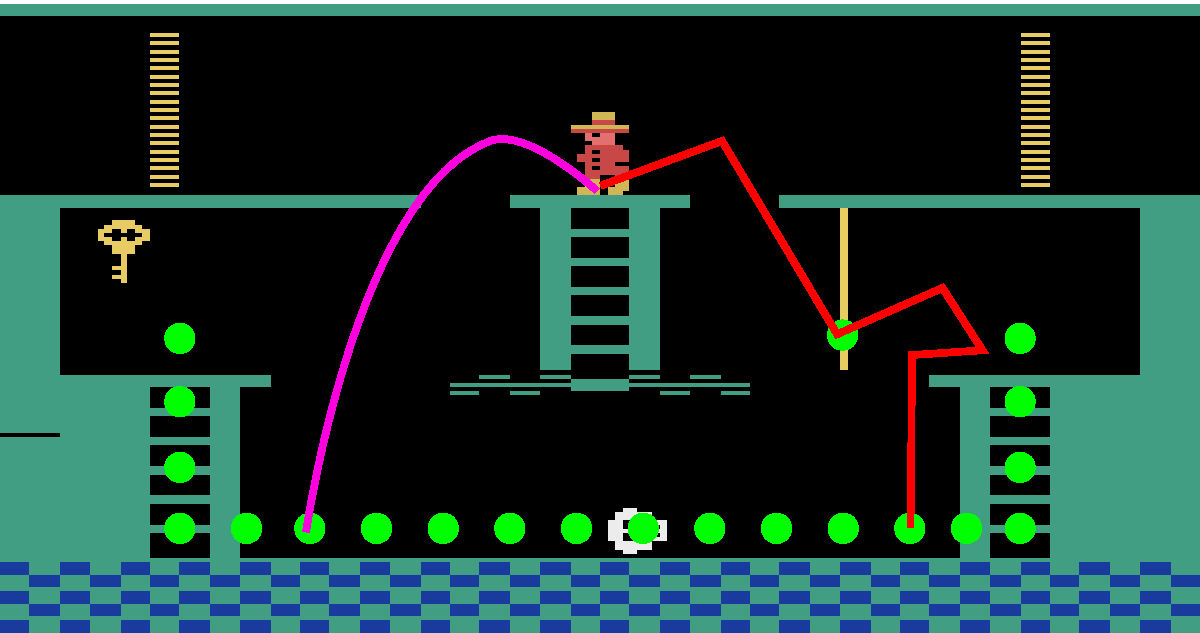
\includegraphics[width=\textwidth / 5 * 3]{img/shaping-defeated.pdf}
\end{center}
\caption{The original shaping rewards, and the two ways the agent found of
  defeating their purpose. First, it took the magenta path. After restricting
  the amount of rewards to be collected at the same time, it took the red
path.\label{fig:shaping-pitfalls}}
\end{figure}

%%% Local Variables: 
%%% mode: latex
%%% TeX-master: "../report"
%%% End: 
\cleardoublepage
\chapter{Conclusions and Future Work}
  \section{Conclusions}
  That a little domain knowledge can go very far
  \section{Future work}
  How we can generalize the results obtained here to other sparse-feedback MDPs.
  Discuss the possible meta-learner

\cleardoublepage
\thispagestyle{empty}
\printbibliography
\addcontentsline{toc}{chapter}{Bibliography}
\end{document}
